% Copyright 2004 by Till Tantau <tantau@users.sourceforge.net>.
%
% In principle, this file can be redistributed and/or modified under
% the terms of the GNU Public License, version 2.
%
% However, this file is supposed to be a template to be modified
% for your own needs. For this reason, if you use this file as a
% template and not specifically distribute it as part of a another
% package/program, I grant the extra permission to freely copy and
% modify this file as you see fit and even to delete this copyright
% notice.

\documentclass{beamer}
\usepackage{graphics}
\usepackage{tikz}
\usepackage{amsfonts}
\usepackage{amsmath}
\usepackage{url}
\usepackage{basicarith}


% There are many different themes available for Beamer. A comprehensive
% list with examples is given here:
% http://deic.uab.es/~iblanes/beamer_gallery/index_by_theme.html
% You can uncomment the themes below if you would like to use a different
% one:
%\usetheme{AnnArbor}
%\usetheme{Antibes}
%\usetheme{Bergen}
%\usetheme{Berkeley}
%\usetheme{Berlin}
%\usetheme{Boadilla}
%\usetheme{boxes}
%\usetheme{CambridgeUS}
%\usetheme{Copenhagen}
%\usetheme{Darmstadt}
%\usetheme{default}
%\usetheme{Frankfurt}
%\usetheme{Goettingen}
%\usetheme{Hannover}
%\usetheme{Ilmenau}
%\usetheme{JuanLesPins}
%\usetheme{Luebeck}
\usetheme{Madrid}
%\usetheme{Malmoe}
%\usetheme{Marburg}
%\usetheme{Montpellier}
%\usetheme{PaloAlto}
%\usetheme{Pittsburgh}
%\usetheme{Rochester}
%\usetheme{Singapore}
%\usetheme{Szeged}
%\usetheme{Warsaw}

\title{Numbers in Non-Integer Bases}

\author[Connor Baker]{Connor Baker \qquad Dr. Tyler White}
% - Give the names in the same order as the appear in the paper.
% - Use the \inst{?} command only if the authors have different
%   affiliation.

\institute[NVCC]{Northern Virginia Community College} % (optional, but mostly needed)

\date{VMATYC, Spring 2017}
% - Either use conference name or its abbreviation.
% - Not really informative to the audience, more for people (including
%   yourself) who are reading the slides online

\subject{Number Theory}
% This is only inserted into the PDF information catalog. Can be left
% out.

% If you have a file called "university-logo-filename.xxx", where xxx
% is a graphic format that can be processed by latex or pdflatex,
% resp., then you can add a logo as follows:

% \pgfdeclareimage[height=0.5cm]{university-logo}{university-logo-filename}
% \logo{\pgfuseimage{university-logo}}

% Delete this, if you do not want the table of contents to pop up at
% the beginning of each subsection:
\AtBeginSubsection[]
{
\begin{frame}<beamer>{Overview}
  \tableofcontents[currentsection,currentsubsection]
\end{frame}
}

% Let's get started
\begin{document}

\begin{frame}
  \titlepage
\end{frame}

\begin{frame}{Outline}
  \tableofcontents
  % You might wish to add the option [pausesections]
\end{frame}










%%%%%%%%%%%%%%%%%%%%%%%%%%%%%%%%%%%%%%%%%%%%%%%%%%%%%%%%%%%%%%%%%%
%%                       WHOLE NUMBERS                          %%
%%%%%%%%%%%%%%%%%%%%%%%%%%%%%%%%%%%%%%%%%%%%%%%%%%%%%%%%%%%%%%%%%%
\section{Whole Numbers}










%%%%%%%%%%%%%%%%%%%%%%%%%%%%%%%%%%%%%%%%%%%%%%%%%%%%%%%%%%%%%%%%%%
%%                        DEFINITIONS                           %%
%%%%%%%%%%%%%%%%%%%%%%%%%%%%%%%%%%%%%%%%%%%%%%%%%%%%%%%%%%%%%%%%%%
\subsection{Definitions}
\begin{frame}{Definition}
  \begin{block}{Base}
    A base (or radix) is a mathematical building block used to describe a number system whose digits are used to represent numbers.
  \end{block}\pause

  \begin{example}[Different Whole Number Bases]\pause
    $125_{10}$ \pause

    $888_9$ \pause

    $48.5_8$ \pause ?
  \end{example}
\end{frame}

\begin{frame}{Definition}
  \begin{block}{Maximum Allowed Numeral in Base}
    The radix is the number of numerals allowed in a base, and it includes zero. \pause

    The number of numerals in a base is one less than the base.
  \end{block}\pause

  \begin{example}[Allowed Numbers in Different Bases]\pause
    $125_{10}$ \pause

    $888_9$ \pause

    $48.5_8$
  \end{example}
\end{frame}
% Corrected version of above slide with purposeful base typo
\begin{frame}{Definition}
  \addtocounter{framenumber}{-1}
  \begin{block}{Maximum Allowed Numeral in Base}
    The radix is the number of numerals allowed in a base, and it includes zero.

    The number of numerals in a base is one less than the base.
  \end{block}

  \begin{example}[Allowed Numbers in Different Bases]
    $125_{10}$

    $888_9$

    $48.5_9$
  \end{example}
\end{frame}

\begin{frame}{Definition}
  \begin{block}{Radix Point}
    A point used to separate the integer part of a number from the fractional part.
  \end{block}\pause

  \begin{example}[Radix Point Expressions]\pause
      $10.5_{10}$ \pause

      A5.E$_{16}$ \pause

      $1.1_2$
  \end{example}
\end{frame}

\begin{frame}{Definition}
  \begin{block}{Beta Expansion}
    A means of rewriting a number as the digits multiplied by the base which is raised to the power of position of the digit.
  \end{block}\pause

  \begin{example}[Example of Beta Expansions]\pause
    $125_{10} = 1\times10^2 + 2\times10^1 + 5\times10^0$ \pause

    A5.E$_{16} = 10\times16^1 + 5\times16^0 + 14\times16^{-1}$ \pause

    $20_2 = 2\times10^1+0\times2^0$
  \end{example}
\end{frame}








%%%%%%%%%%%%%%%%%%%%%%%%%%%%%%%%%%%%%%%%%%%%%%%%%%%%%%%%%%%%%%%%%%
%%                          EXAMPLES                            %%
%%%%%%%%%%%%%%%%%%%%%%%%%%%%%%%%%%%%%%%%%%%%%%%%%%%%%%%%%%%%%%%%%%
\subsection{Examples}
\begin{frame}{Let's Play a Game}
\begin{itemize}
  \item Suppose that you're given the interval $[0,1]$, with a point somewhere on it \pause
  \begin{center}
    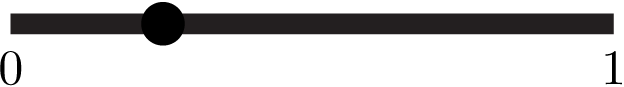
\includegraphics{images/interval/intervalwithdot}
  \end{center} \pause
    \item You're allowed one operation
    \begin{itemize}
      \item Multiplication by a whole number, followed by modulo one \pause
      \item Once you choose a multiplier, you must use it for the duration \pause
    \end{itemize}
    \item We keep track of the interval that it falls in after the operation
  \end{itemize}
\end{frame}

\begin{frame}{Dealing with Radix Point Expressions (Geometrically)}
  \begin{example}[Suppose you have a point...]
    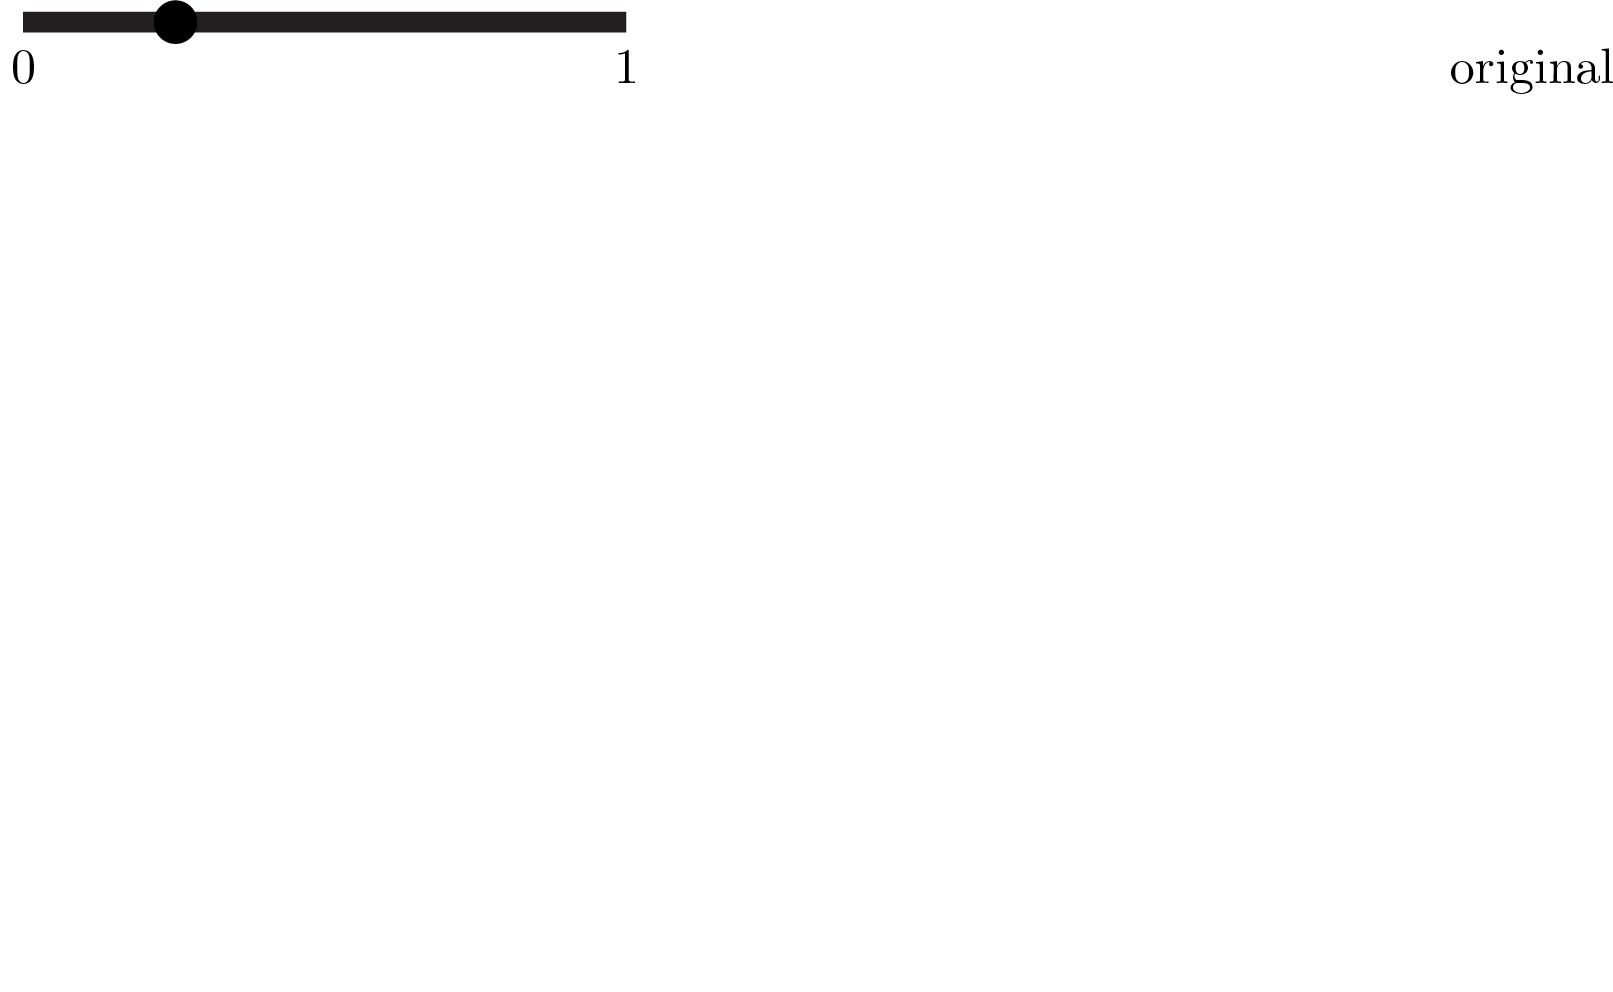
\includegraphics[width=\textwidth,height=0.75\textheight]{images/Binary/1}
  \end{example}
\end{frame}

\begin{frame}{Dealing with Radix Point Expressions (Geometrically)}
  \addtocounter{framenumber}{-1}
  \begin{example}[Suppose you have a point...]
    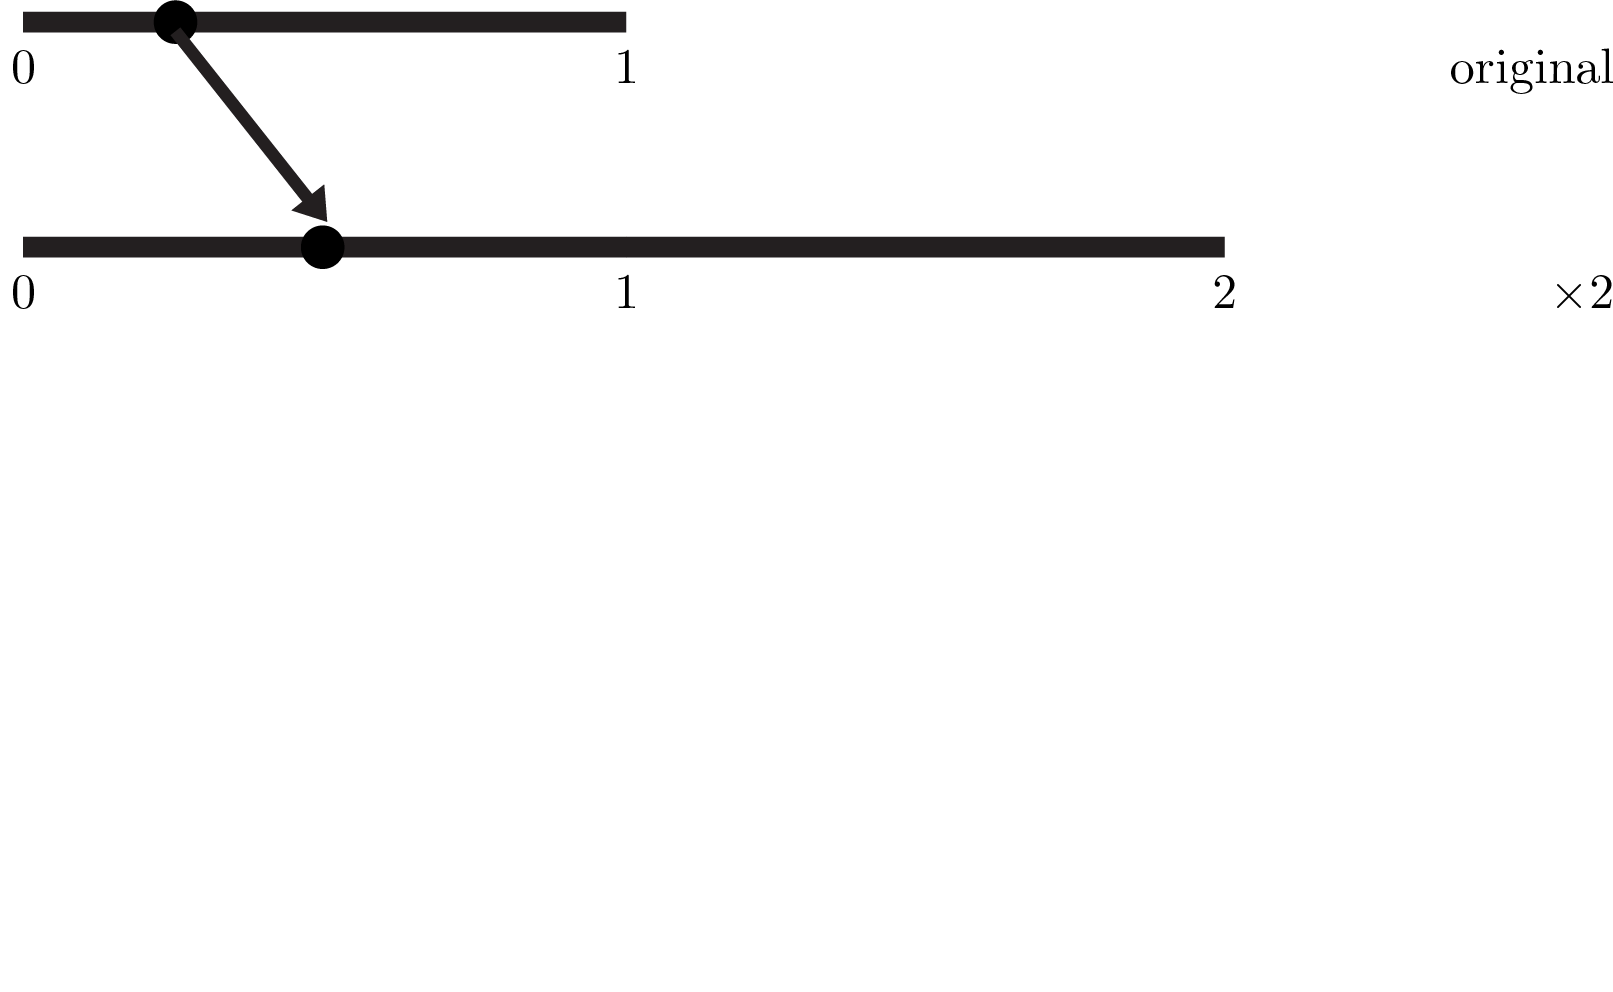
\includegraphics[width=\textwidth,height=0.75\textheight]{images/Binary/2}
  \end{example}
\end{frame}

\begin{frame}{Dealing with Radix Point Expressions (Geometrically)}
  \addtocounter{framenumber}{-1}
  \begin{example}[Suppose you have a point...]
    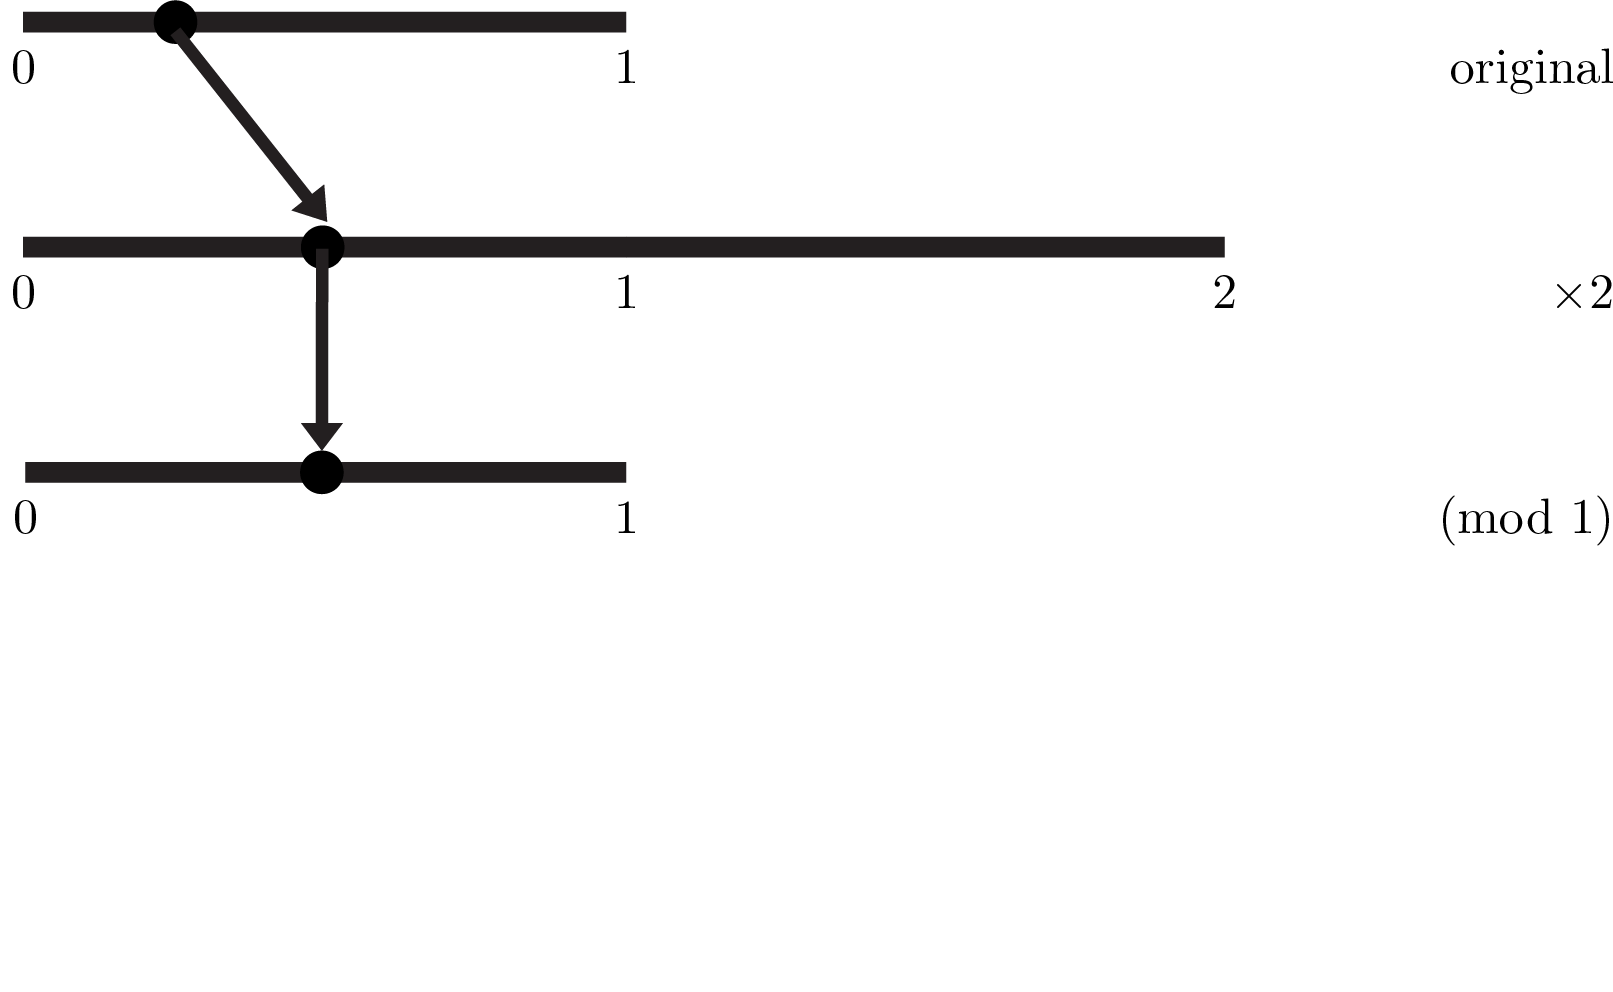
\includegraphics[width=\textwidth,height=0.75\textheight]{images/Binary/3}
  \end{example}
\end{frame}

\begin{frame}{Dealing with Radix Point Expressions (Geometrically)}
  \addtocounter{framenumber}{-1}
  \begin{example}[Suppose you have a point...]
    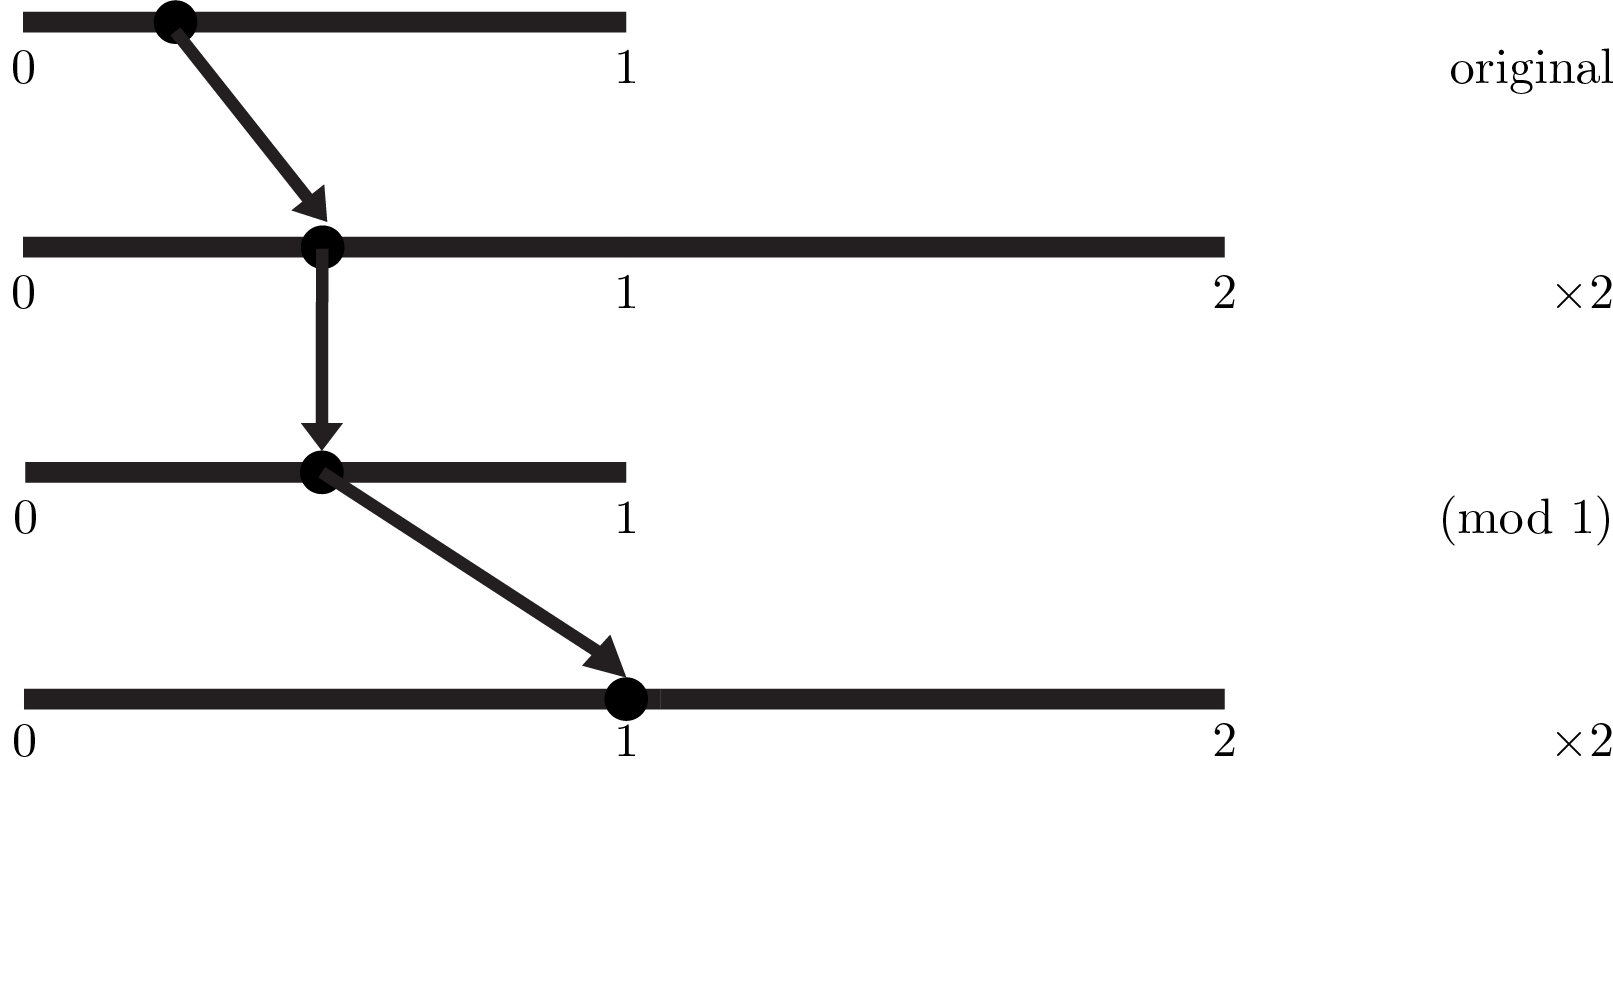
\includegraphics[width=\textwidth,height=0.75\textheight]{images/Binary/4}
  \end{example}
\end{frame}

\begin{frame}{Dealing with Radix Point Expressions (Geometrically)}
  \addtocounter{framenumber}{-1}
  \begin{example}[Suppose you have a point...]
    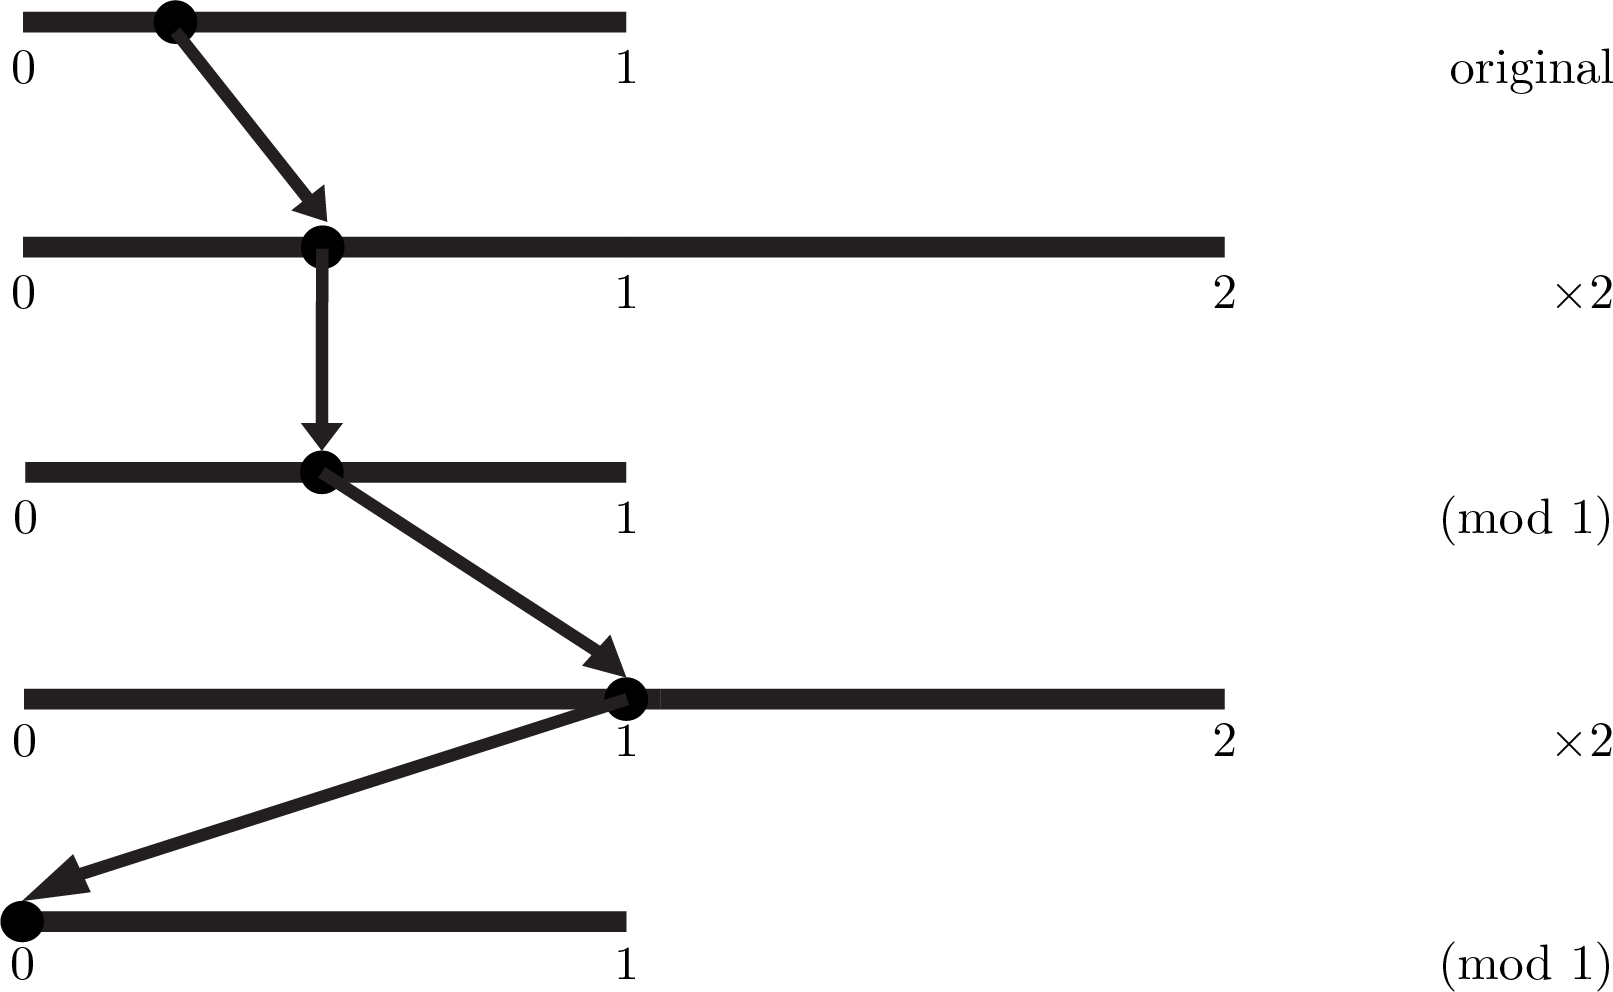
\includegraphics[width=\textwidth,height=0.75\textheight]{images/Binary/5}
  \end{example}
\end{frame}

\begin{frame}{How Partitioning Works}
  \begin{itemize}
    \item We partition before we multiply \pause
    \item We multiply so that the first partition becomes the unit interval \pause
    \begin{itemize}
      \item The number we multiply by is the base that we are converting to \pause
    \end{itemize}
    \item So for binary, this is what we were doing:
  \end{itemize}
  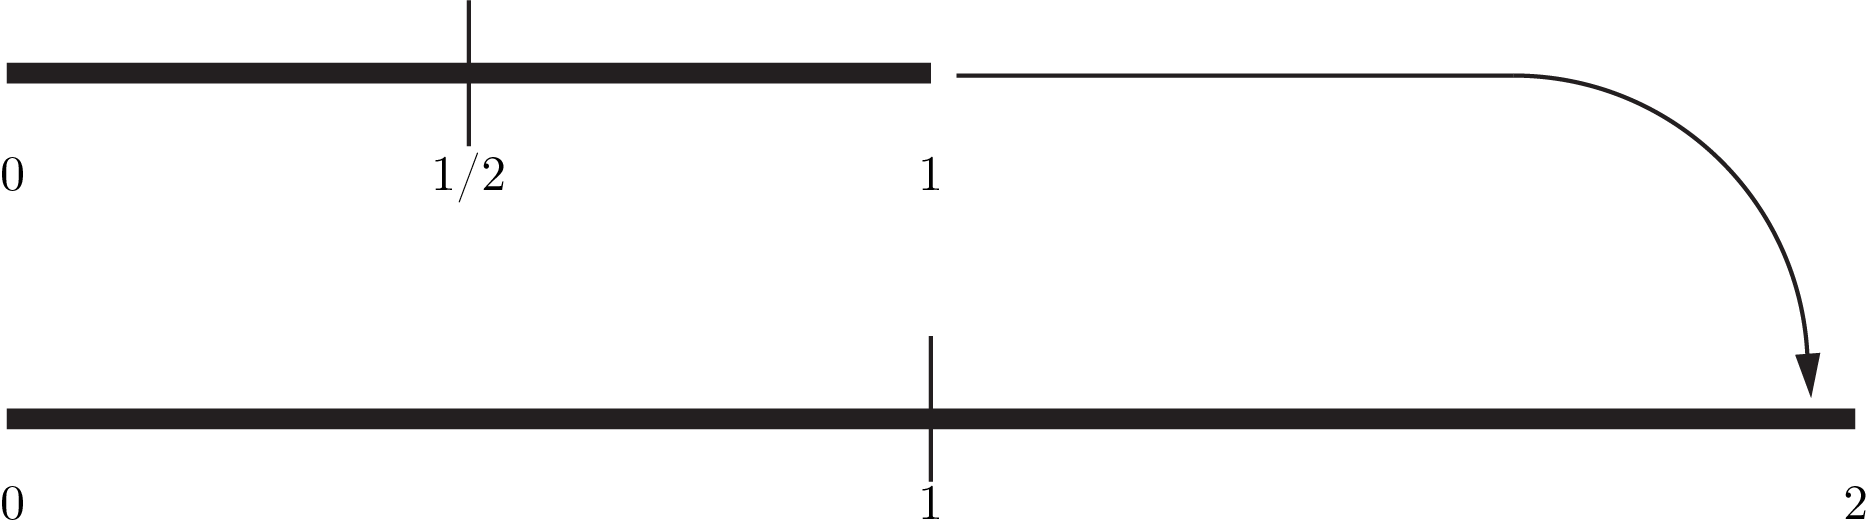
\includegraphics[width=\textwidth]{images/partitioning/partitioning}
\end{frame}

\begin{frame}{What this Tells Us}
  \begin{itemize}
    \item Where the point was originally \pause
    \begin{itemize}
      \item The conversion of $0.25_{10}$ to a number in binary: $0.01_2$
      \item We can check this with a beta expansion: $0.01_2 = 0\times2^{0} + 0\times2^{-1} + 1\times2^{-2} = 1/4 = 0.25_{10}$
    \end{itemize} \pause
  \item That there is a finite radix point expression in a given base \pause
  \item That our choice of partitioning and multiplication matter... this is what happens geometrically when we change bases \pause
  \item Let's do another example
  \end{itemize}
\end{frame}

\begin{frame}{Dealing with Radix Point Expressions (Geometrically)}
  \begin{example}[Suppose you have a point...]
    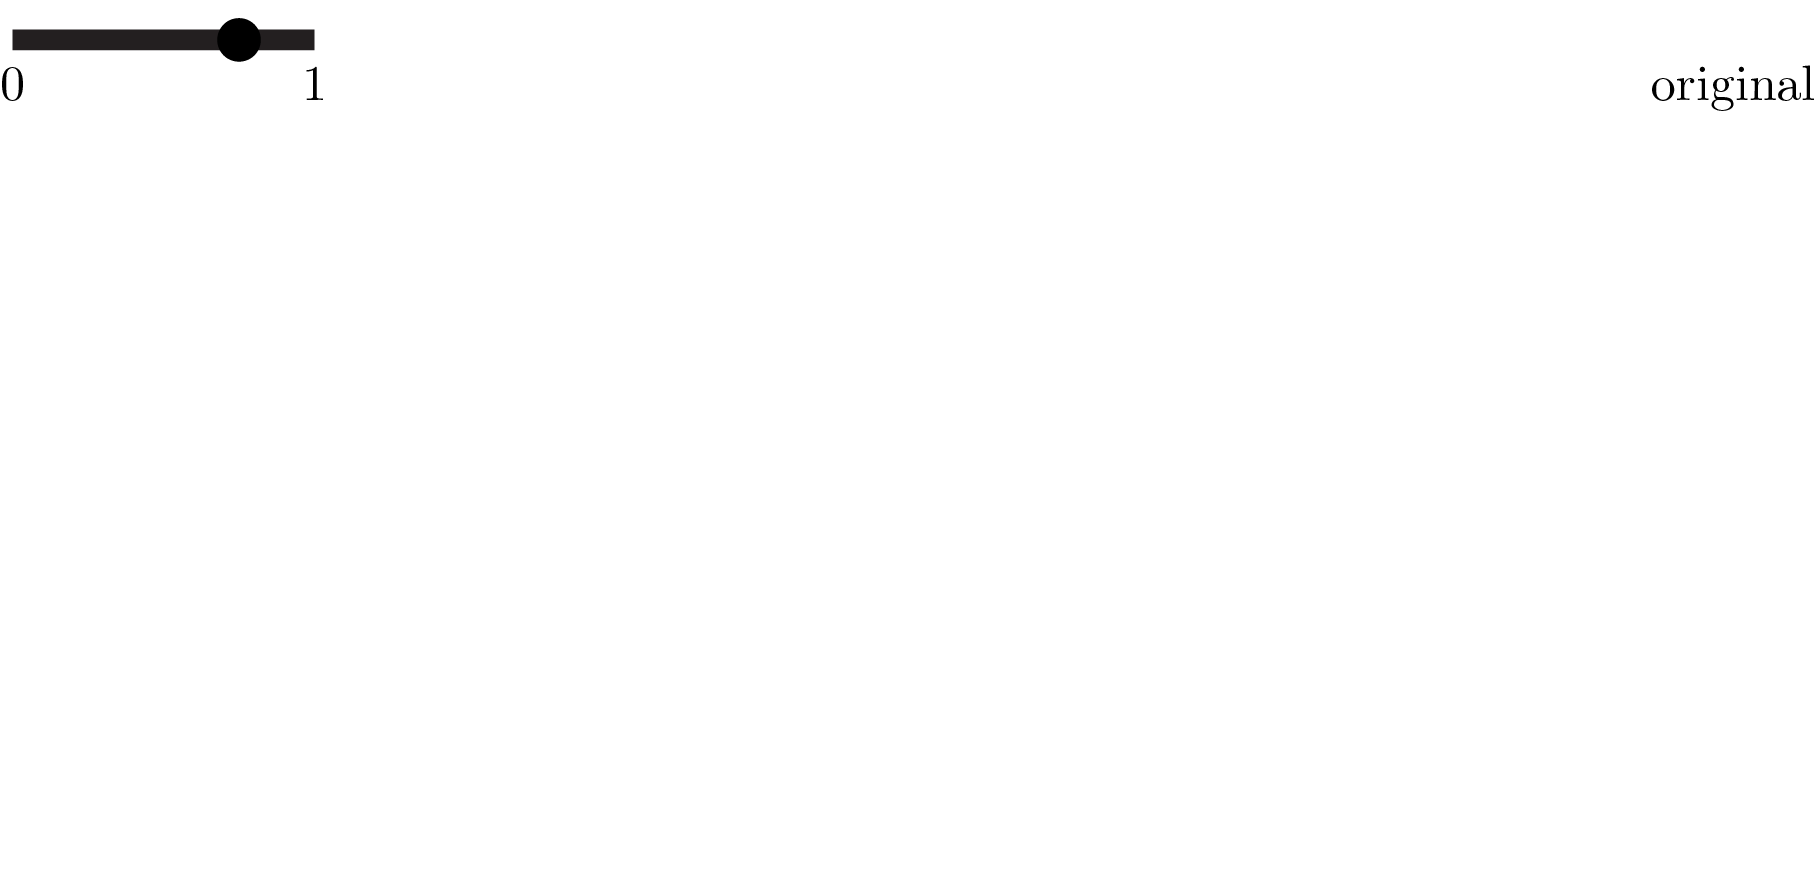
\includegraphics[width=\textwidth,height=0.75\textheight]{images/Ternary/1}
  \end{example}
\end{frame}

\begin{frame}{Dealing with Radix Point Expressions (Geometrically)}
  \addtocounter{framenumber}{-1}
  \begin{example}[Suppose you have a point...]
    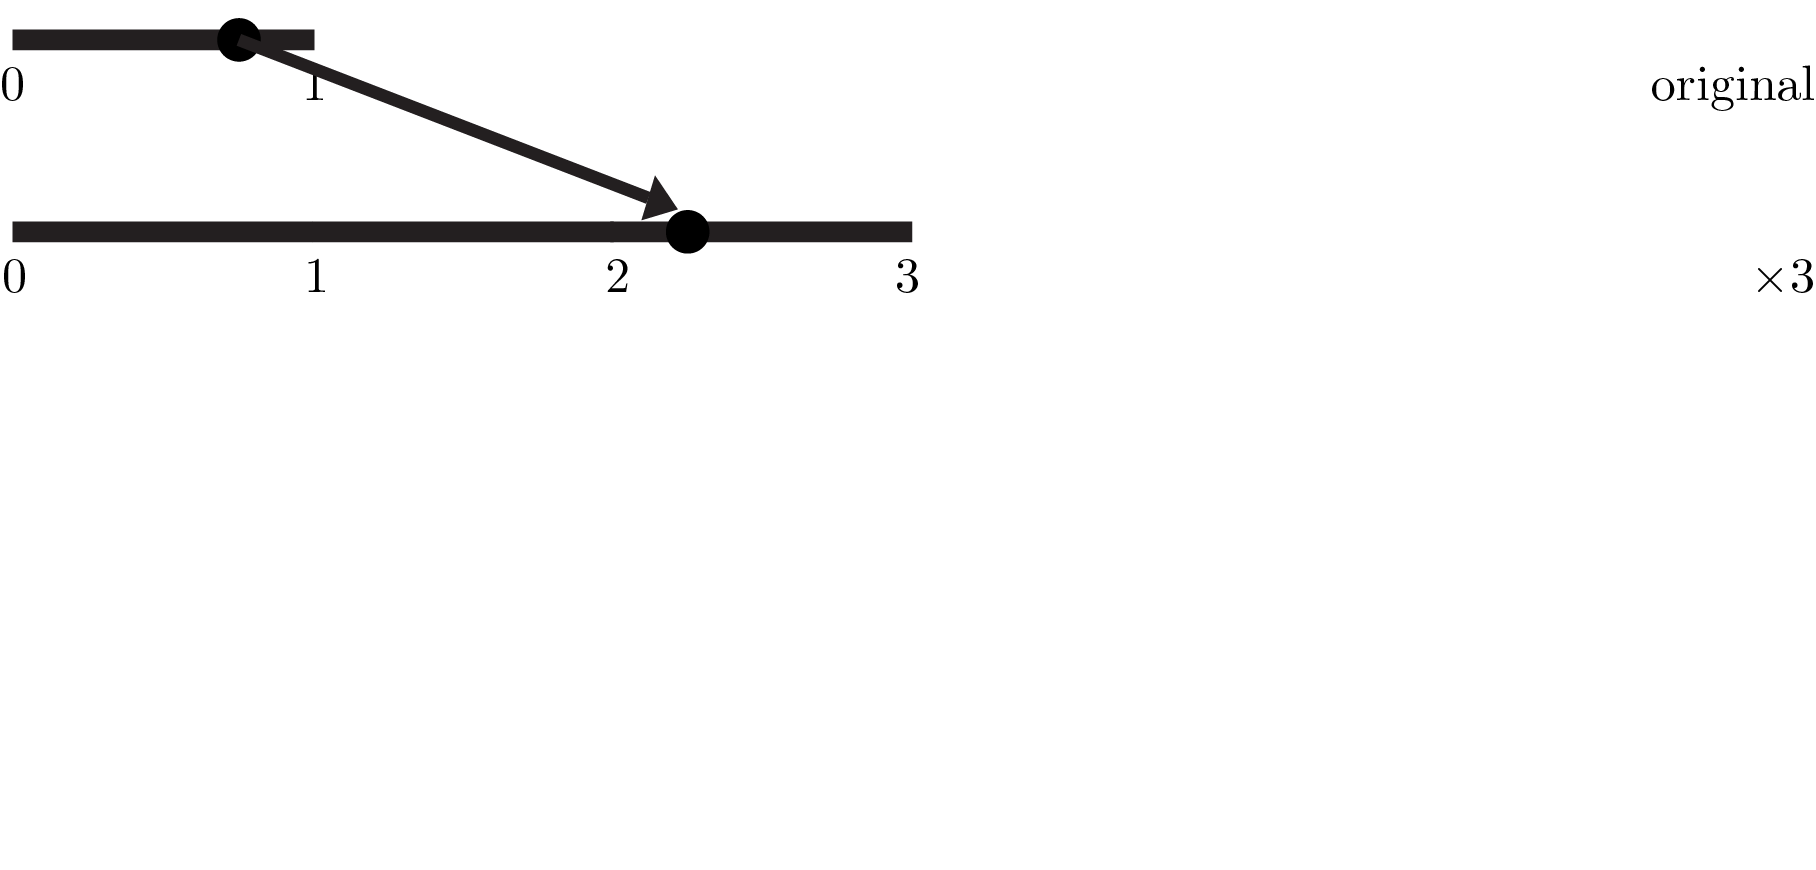
\includegraphics[width=\textwidth,height=0.75\textheight]{images/Ternary/2}
  \end{example}
\end{frame}

\begin{frame}{Dealing with Radix Point Expressions (Geometrically)}
  \addtocounter{framenumber}{-1}
  \begin{example}[Suppose you have a point...]
    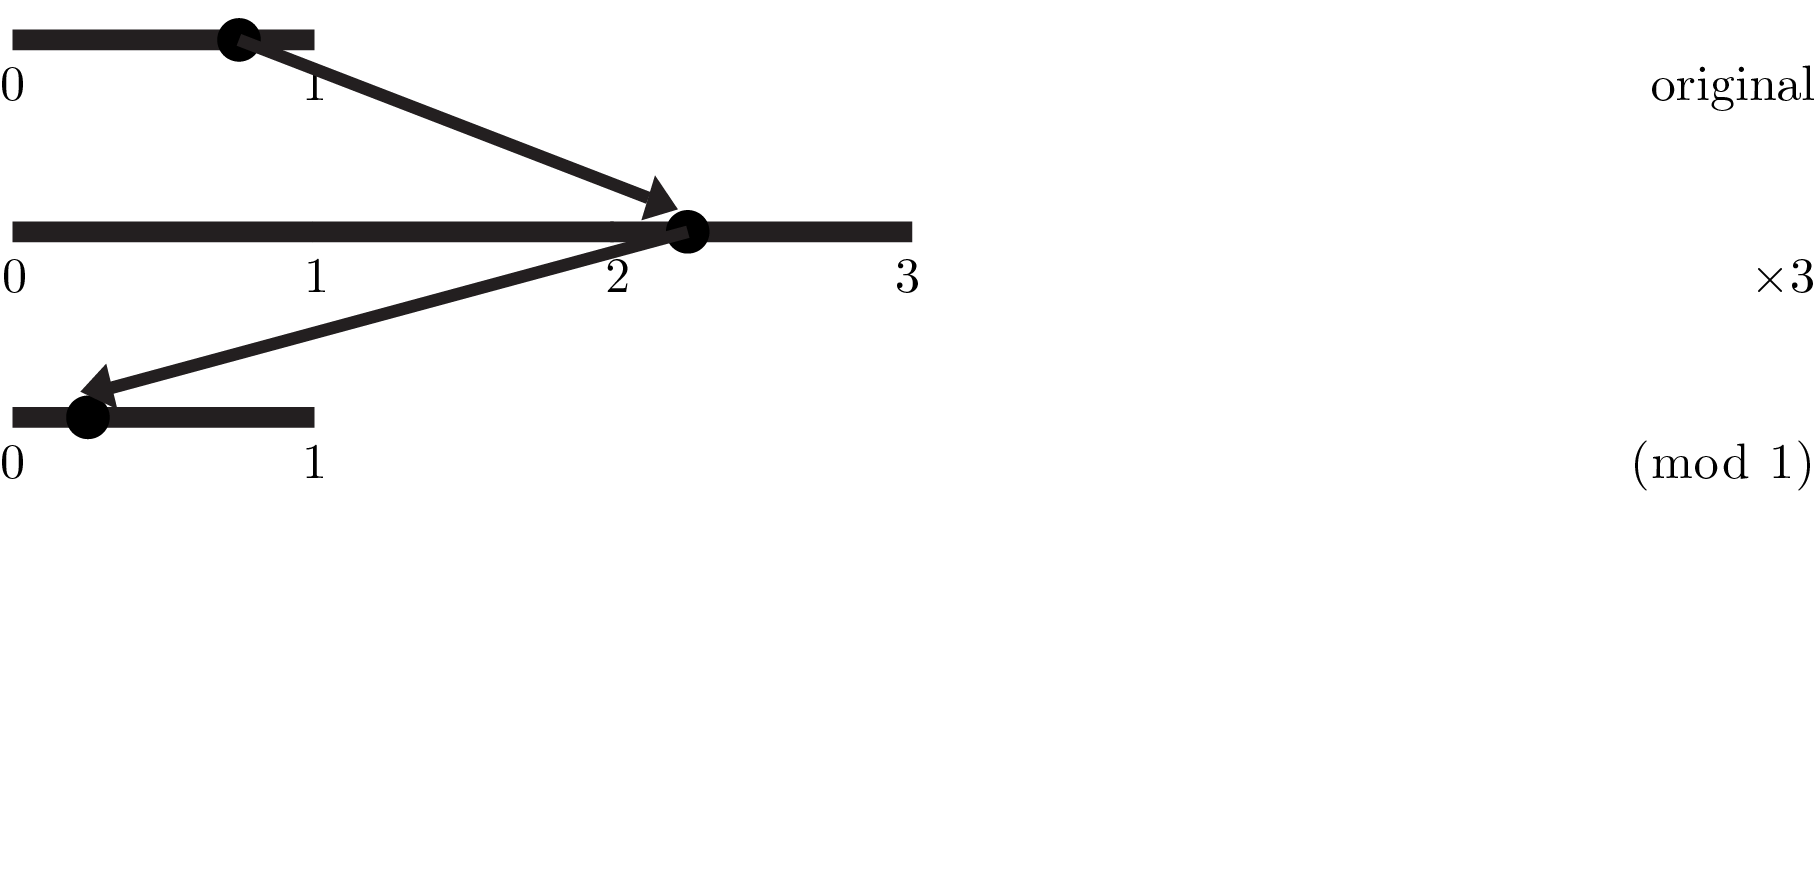
\includegraphics[width=\textwidth,height=0.75\textheight]{images/Ternary/3}
  \end{example}
\end{frame}

\begin{frame}{Dealing with Radix Point Expressions (Geometrically)}
  \addtocounter{framenumber}{-1}
  \begin{example}[Suppose you have a point...]
    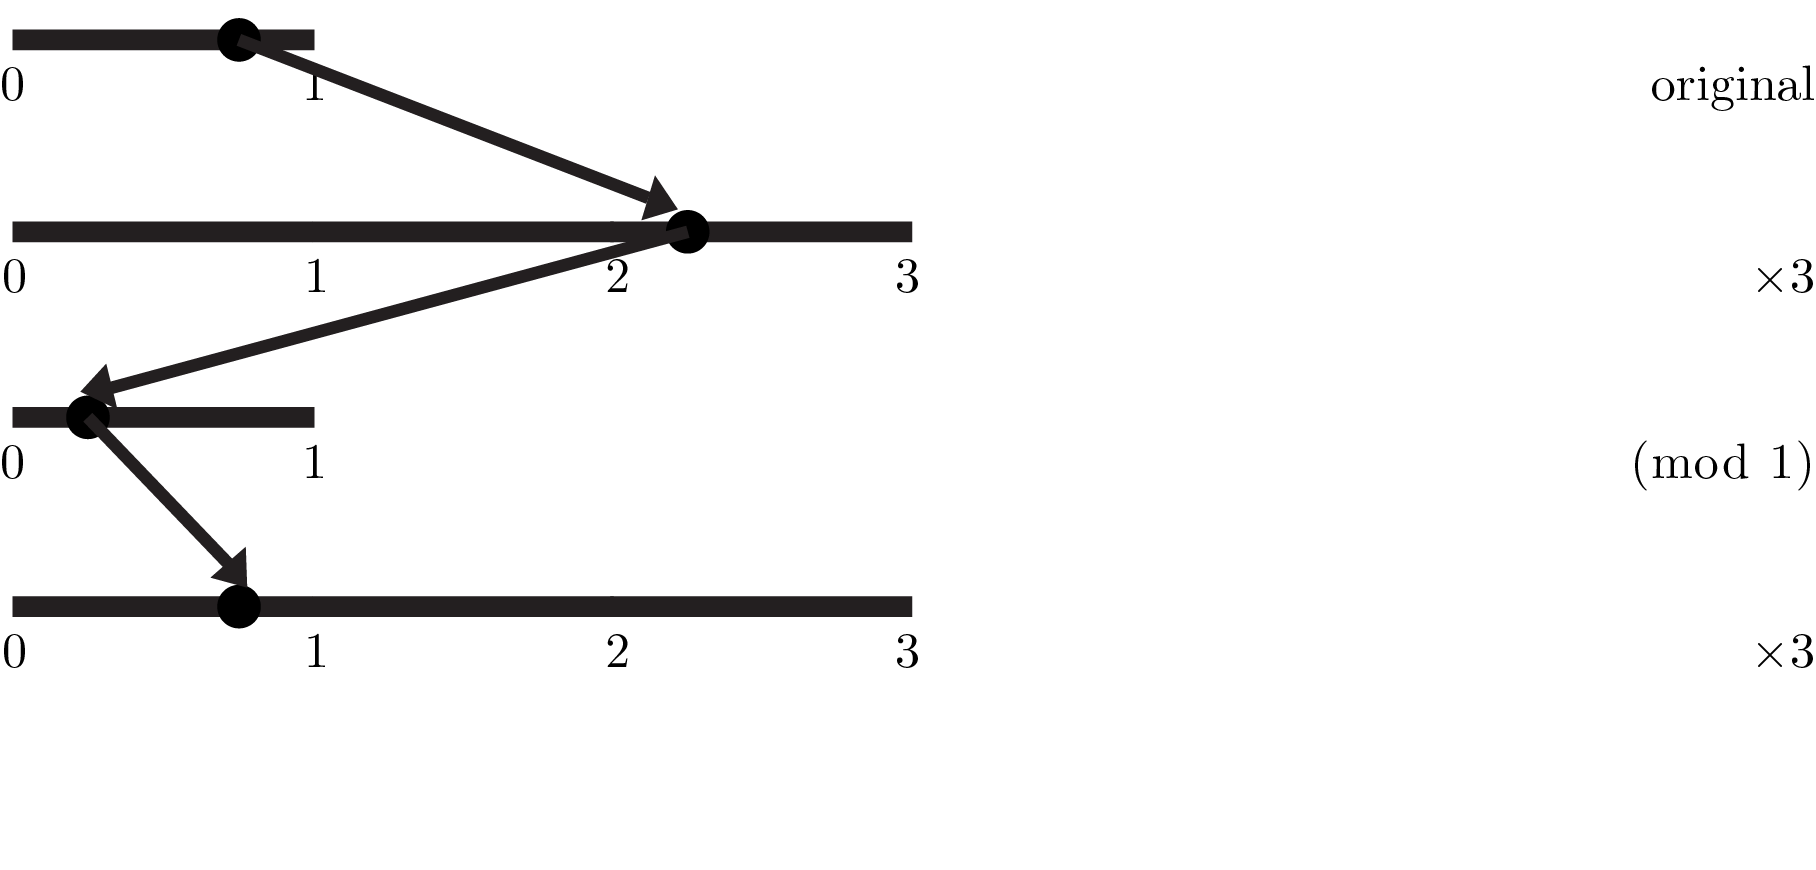
\includegraphics[width=\textwidth,height=0.75\textheight]{images/Ternary/4}
  \end{example}
\end{frame}

\begin{frame}{Dealing with Radix Point Expressions (Geometrically)}
  \addtocounter{framenumber}{-1}
  \begin{example}[Suppose you have a point...]
    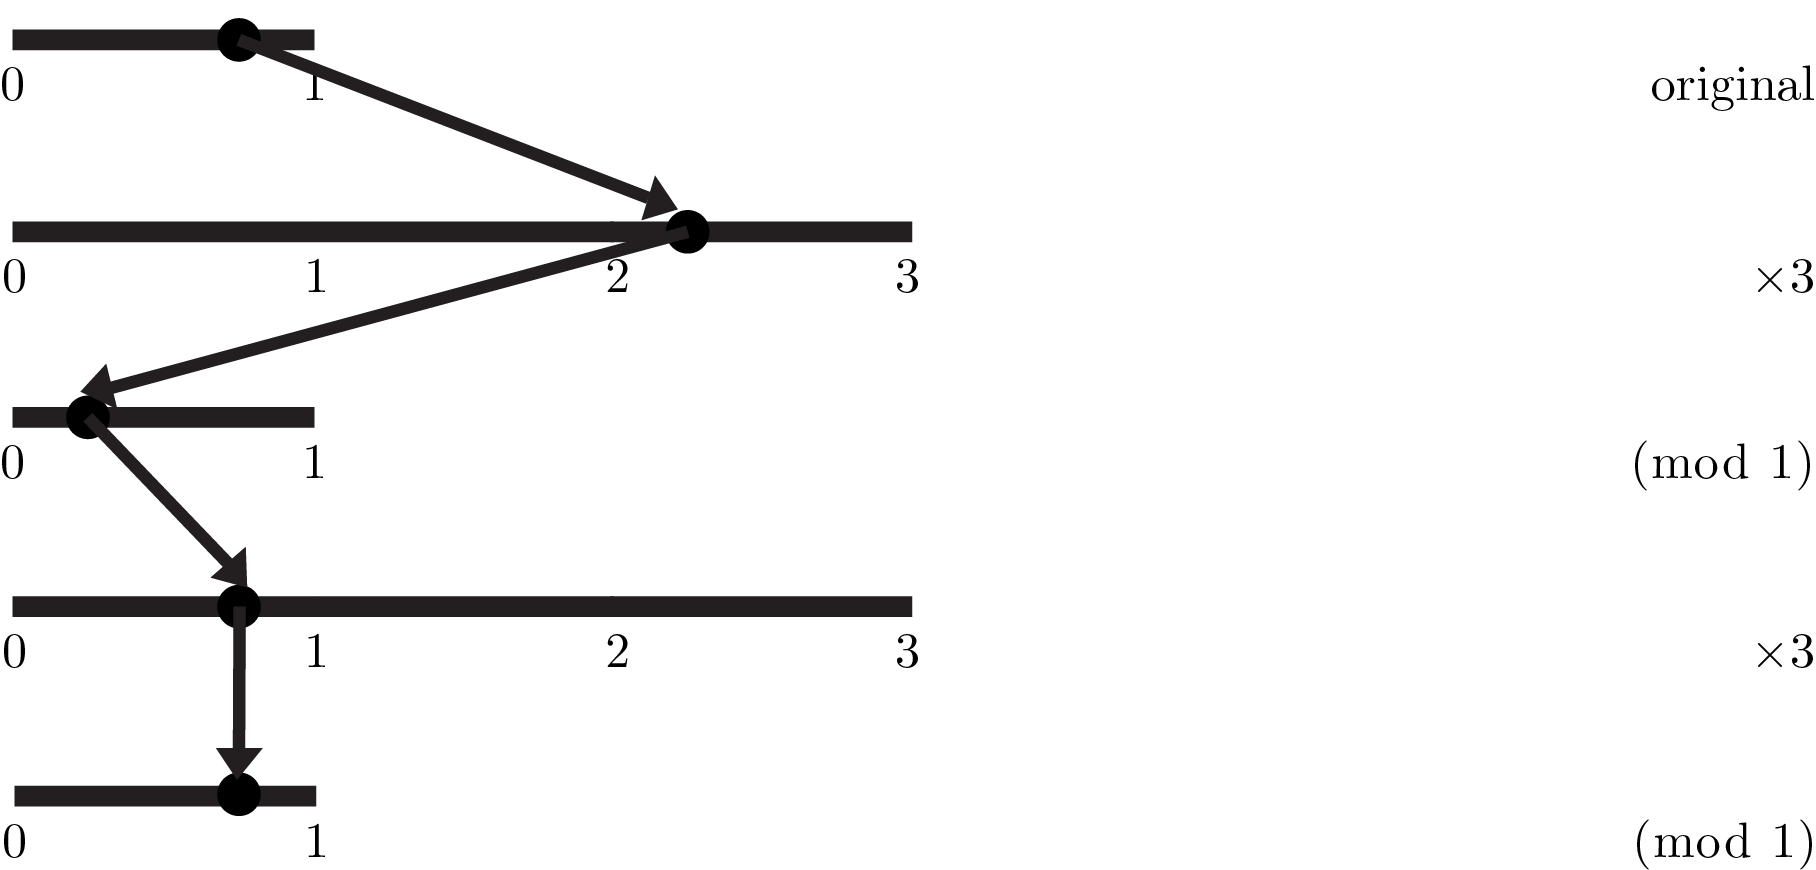
\includegraphics[width=\textwidth,height=0.75\textheight]{images/Ternary/5}
  \end{example}
\end{frame}

\begin{frame}{Dealing with Radix Point Expressions (Geometrically)}
  \addtocounter{framenumber}{-1}
  \begin{example}[Suppose you have a point...]
    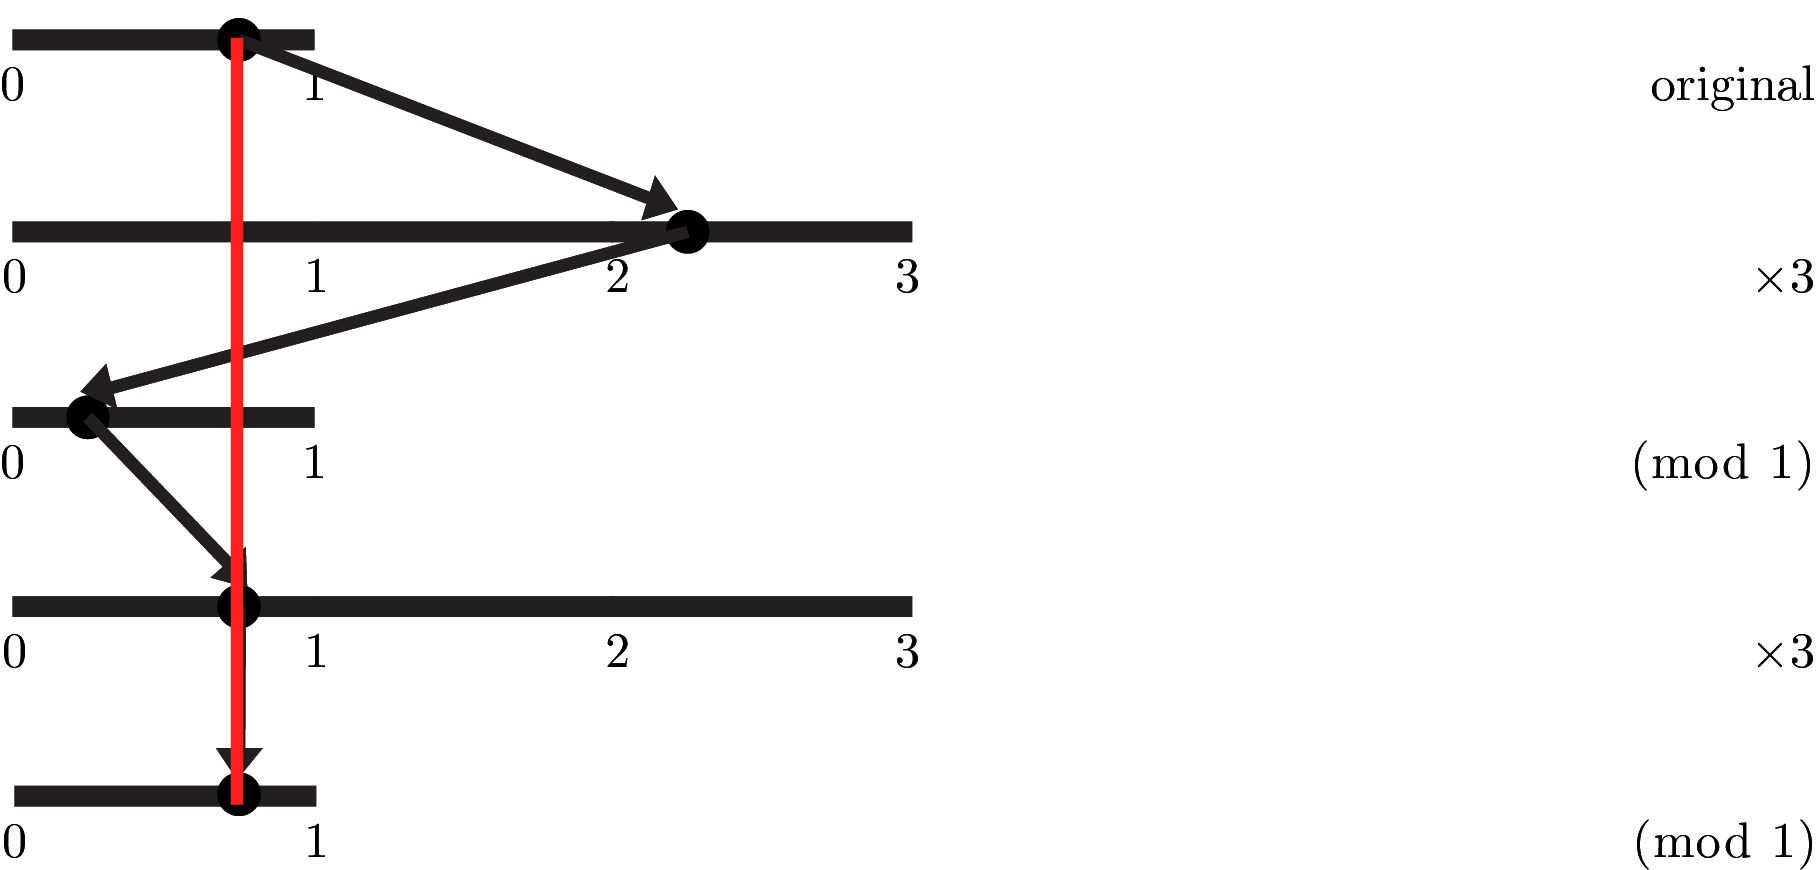
\includegraphics[width=\textwidth,height=0.75\textheight]{images/Ternary/6}
  \end{example}
\end{frame}

\begin{frame}{What this Tells Us}
  \begin{itemize}
    \item Getting stuck in this cycle means this number is not representable as a finite radix point expression in base 3 \pause
    \item In general, this can and does happen in any base \pause
    \item We can explain this phenomenon arithmetically
  \end{itemize}
\end{frame}

\begin{frame}{Theorem}
  \begin{block}{Finite Radix Point Expression} \pause
    A number $p$ is said to have a finite radix point expression if $$p=\frac{n}{m_1 m_2\dots m_k}$$ where $n\in\mathbb{N}$, and $m_1 m_2 \dots m_k$ are all the prime factors of the base raised to some power. \footnotetext{\url{http://mathworld.wolfram.com/DecimalExpansion.html}}
  \end{block}\pause

  \begin{example}[1/3 in Base 10]
    $$\frac{1}{3} \neq \frac{n}{2^\alpha 5^\beta}$$

    where $n,\alpha,\beta\in\mathbb{N}$.
  \end{example}
\end{frame}

\begin{frame}{Dealing with Radix Point Expressions (Arithmetically)}
  \begin{itemize}
    \item We can do this operation with arithmetic \pause
      \begin{itemize}
        \item We must first qualify what we were doing in our $``$game" previously
      \end{itemize}
  \end{itemize}
\end{frame}


\begin{frame}{Definition}
  \begin{block}{Beta Map}
    The transformation $T:[0,1)\to[0,1)$ defined by $T=(x\cdot\beta)\pmod{1}$.
  \end{block}
\end{frame}

\begin{frame}{Dealing with Radix Point Expressions (Arithmetically)}
  \begin{example}[Convert $0.1_{10}$ to binary.]\pause
    \begin{enumerate}
      \item[] 0.1 * 2 = 0.2 \qquad 0.2 mod (1) = 0.2 \hfill 0.0\pause
      \item[] 0.2 * 2 = 0.4 \qquad 0.4 mod (1) = 0.4 \hfill 0.00\pause
      \item[] 0.4 * 2 = 0.8 \qquad 0.8 mod (1) = 0.8 \hfill 0.000\pause
      \item[] 0.8 * 2 = 1.6 \qquad 1.6 mod (1) = 0.6 \hfill 0.0001\pause
      \item[] 0.6 * 2 = 1.2 \qquad 1.2 mod (1) = 0.2 \hfill 0.00011\pause
      \item[] 0.2 * 2 = 0.4 \qquad 0.4 mod (1) = 0.4 \hfill\dots\pause
    \end{enumerate}
    \hfill $0.0\overline{0011}_2$
  \end{example}
\end{frame}















%%%%%%%%%%%%%%%%%%%%%%%%%%%%%%%%%%%%%%%%%%%%%%%%%%%%%%%%%%%%%%%%%%
%%           LANGUAGE GENERATED BY WHOLE NUMBER BASES           %%
%%%%%%%%%%%%%%%%%%%%%%%%%%%%%%%%%%%%%%%%%%%%%%%%%%%%%%%%%%%%%%%%%%
\subsection{Language Generated by Whole Number Bases}
\begin{frame}{Definition}
  \begin{block}{Word}
    A word is a sequence of characters from an alphabet.
  \end{block}\pause

  \begin{example}[Examples of Words] \pause
    101 (Binary) \pause

    99.9 (Decimal)
  \end{example}
\end{frame}

\begin{frame}{Definition}
  \begin{block}{Language}
    A language is the set of all allowed words.
  \end{block}\pause

  \begin{example}[Examples of Languages]\pause
    Binary \pause

    Ternary \pause

    Numerical Bases
  \end{example}
\end{frame}

\begin{frame}{Language Generated by Whole Number Bases}
  \begin{itemize}
    \item A word is not allowed in a language if it contains a forbidden subword \pause
    \begin{itemize}
      \item Acceptable words in base 10 include 9, or 5.5 -- but not CAT or 5Z: they contain forbidden subwords \pause
      \item Acceptable words in base 2 include 1, or 0.110000 -- but not 3, or 4: they contain forbidden subwords
    \end{itemize}\pause
    \item How can we represent the language generated by these bases?
  \end{itemize}
\end{frame}

\begin{frame}{Definition}
  \begin{block}{Finite State Machine}
    A finite state machine (FSM) is a mathematical structure that allows us to imagine a machine with no memory.
  \end{block}
\end{frame}

\begin{frame}{FSM for Binary}
  \begin{center}
    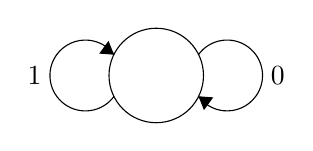
\begin{tikzpicture}[scale=0.2]
      \tikzstyle{every node}+=[inner sep=0pt]
      \draw [black] (38.8,-28) circle (3);
      \draw [black] (41.48,-26.677) arc (144:-144:2.25);
      \draw (46.05,-28) node [right] {$0$};
      \fill [black] (41.48,-29.32) -- (41.83,-30.2) -- (42.42,-29.39);
      \draw [black] (36.12,-29.323) arc (324:36:2.25);
      \draw (31.55,-28) node [left] {$1$};
      \fill [black] (36.12,-26.68) -- (35.77,-25.8) -- (35.18,-26.61);
    \end{tikzpicture}
  \end{center}
\end{frame}

\begin{frame}{FSM for Ternary}
  \begin{center}
    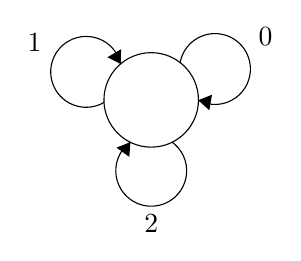
\begin{tikzpicture}[scale=0.2]
      \tikzstyle{every node}+=[inner sep=0pt]
      \draw [black] (38.8,-28) circle (3);
      \draw [black] (40.635,-25.642) arc (169.84114:-118.15886:2.25);
      \draw (45.58,-23.98) node [right] {$0$};
      \fill [black] (41.79,-28.02) -- (42.49,-28.66) -- (42.66,-27.67);
      \draw [black] (35.816,-28.153) arc (300.67038:12.67038:2.25);
      \draw (31.87,-24.37) node [left] {$1$};
      \fill [black] (36.86,-25.72) -- (36.89,-24.78) -- (36.02,-25.29);
      \draw [black] (40.123,-30.68) arc (54:-234:2.25);
      \draw (38.8,-35.25) node [below] {$2$};
      \fill [black] (37.48,-30.68) -- (36.6,-31.03) -- (37.41,-31.62);
    \end{tikzpicture}
  \end{center}
\end{frame}

\begin{frame}{Simplified FSM for Ternary}
  \begin{center}
    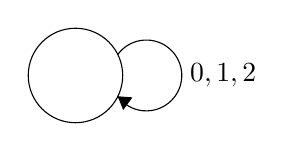
\begin{tikzpicture}[scale=0.2]
      \tikzstyle{every node}+=[inner sep=0pt]
      \draw [black] (38.8,-28) circle (3);
      \draw [black] (41.48,-26.677) arc (144:-144:2.25);
      \draw (46.05,-28) node [right] {$0,1,2$};
      \fill [black] (41.48,-29.32) -- (41.83,-30.2) -- (42.42,-29.39);
    \end{tikzpicture}
  \end{center}
\end{frame}

\begin{frame}{FSM for Whole Number Bases}
  \begin{center}
    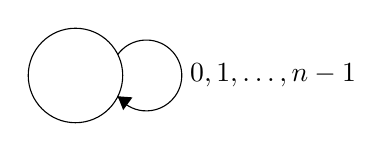
\begin{tikzpicture}[scale=0.2]
      \tikzstyle{every node}+=[inner sep=0pt]
      \draw [black] (38.8,-28) circle (3);
      \draw [black] (41.48,-26.677) arc (144:-144:2.25);
      \draw (46.05,-28) node [right] {$0,1,\dots,n-1$};
      \fill [black] (41.48,-29.32) -- (41.83,-30.2) -- (42.42,-29.39);
    \end{tikzpicture}
  \end{center}
  \begin{itemize}
    \item $n\in\mathbb{N},\ n>1$
  \end{itemize}
\end{frame}
















%%%%%%%%%%%%%%%%%%%%%%%%%%%%%%%%%%%%%%%%%%%%%%%%%%%%%%%%%%%%%%%%%%
%%                     NON-INTEGER NUMBERS                      %%
%%%%%%%%%%%%%%%%%%%%%%%%%%%%%%%%%%%%%%%%%%%%%%%%%%%%%%%%%%%%%%%%%%
\section{Non-Integer Algebraic Numbers}












%%%%%%%%%%%%%%%%%%%%%%%%%%%%%%%%%%%%%%%%%%%%%%%%%%%%%%%%%%%%%%%%%%
%%                          DEFINITIONS                         %%
%%%%%%%%%%%%%%%%%%%%%%%%%%%%%%%%%%%%%%%%%%%%%%%%%%%%%%%%%%%%%%%%%%
\subsection{Definitions}
\begin{frame}{Definition}
  \begin{block}{Maximum Allowed Numeral in Base}
    If the radix is a whole number, the previous definition holds.

    If the radix is not a whole number, then the maximum allowed numeral is the floor function of the base.
  \end{block}\pause

  \begin{example}[Allowed Numbers in Different Bases]\pause
    $\varphi = \frac{1+\sqrt{5}}{2} \approx 1.618$, maximum numeral is 1 \pause

    $\alpha = 1+\sqrt{2} \approx 2.14$, maximum numeral is 2
  \end{example}
\end{frame}

\begin{frame}{Definition}
  \begin{block}{Algebraic Integer}
    A number $x$ is an algebraic integer if it is the root of a monic polynomial $f(x) = x^n + a_{n-1}x^{n-1}+\dots+a_1x+a_0$, where $a_{n-1},\dots,a_0\in\mathbb{Z}$.
  \end{block}

  \begin{example}[Examples of Algebraic Polynomials]\pause
    $$\varphi^2 -\varphi - 1 = 0, \quad x=\frac{1\pm\sqrt{5}}{2}$$\pause

    $$\alpha^2 - 2\alpha - 1 = 0, \quad x = 1\pm\sqrt{2}$$\pause

    $$x^3 -x - 1 = 0, \quad x=\frac{1}{3}\sqrt[3]{\frac{27-3\sqrt{69}}{2}} + \frac{\sqrt[3]{\frac{1}{2}(9 + \sqrt{69})}}{3^{2/3}}$$
  \end{example}
\end{frame}



%%%%%%%%%%%%%%%%%%%%%%%%%%%%%%%%%%%%%%%%%%%%%%%%%%%%%%%%%%%%%%%%%%
%%                 PARTITIONING DIFFERENTLY                    %%
%%%%%%%%%%%%%%%%%%%%%%%%%%%%%%%%%%%%%%%%%%%%%%%%%%%%%%%%%%%%%%%%%%
\begin{frame}{Partitioning Differently}
  \begin{itemize}
    \item We don't have to use a whole number \pause
    \item The partitions won't be even, but that's not a problem \pause
  \end{itemize}
  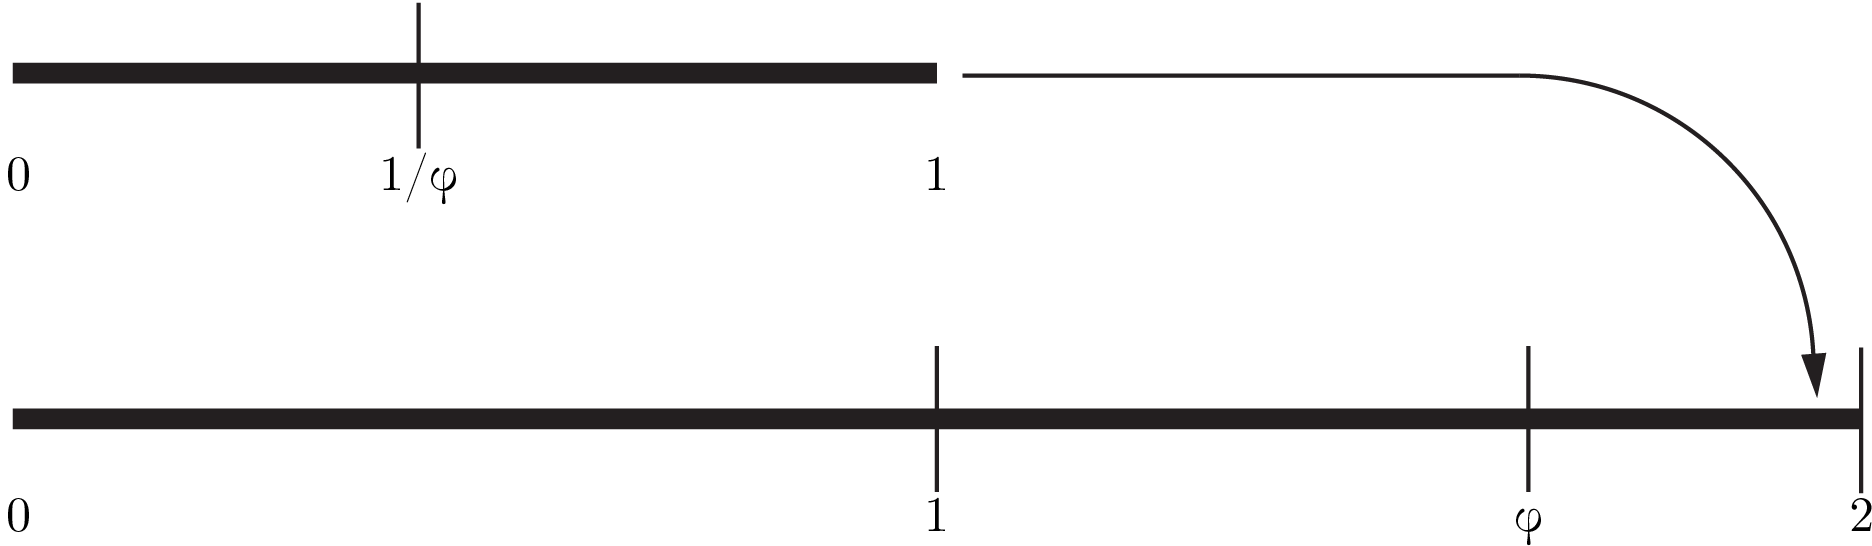
\includegraphics[width=\textwidth]{images/partitioning/partitioningbeta}
\end{frame}

\begin{frame}{Partitioning Differently}
  \addtocounter{framenumber}{-1}
  \begin{itemize}
    \item We don't have to use a whole number
    \item The partitions won't be even, but that's not a problem
  \end{itemize}
  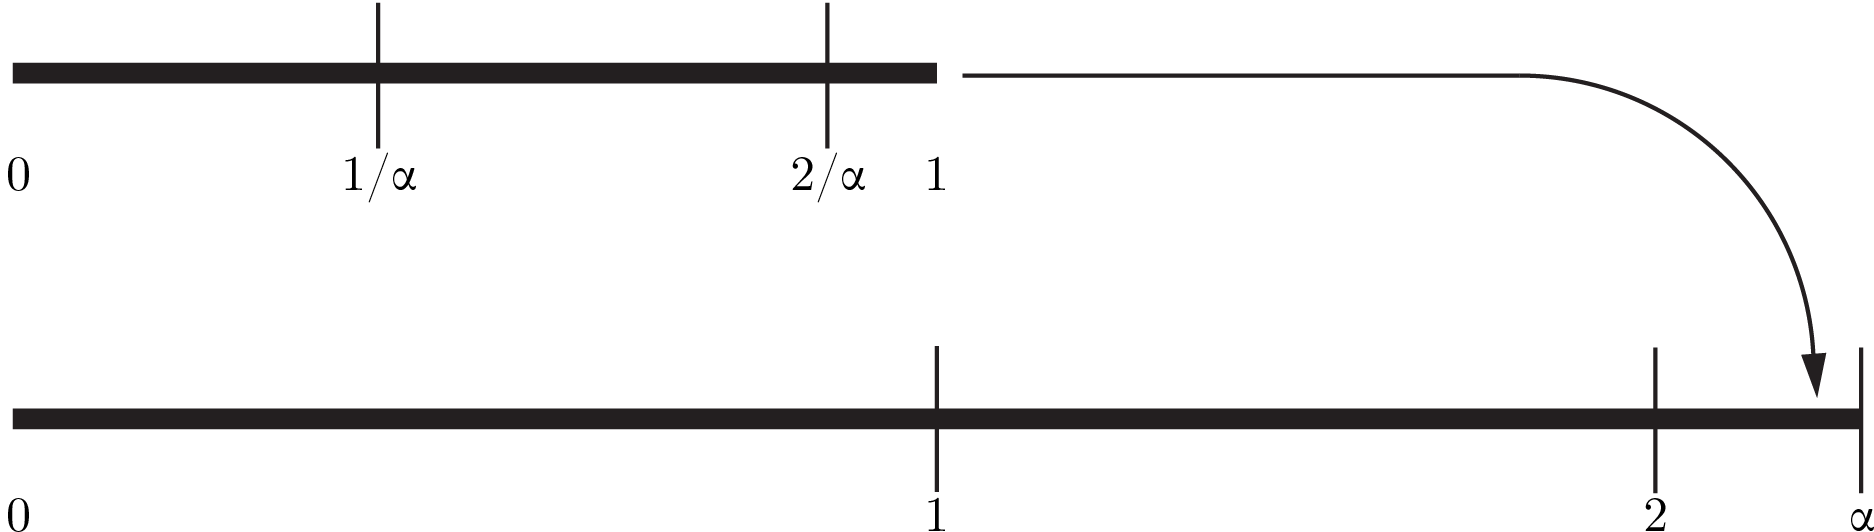
\includegraphics[width=\textwidth]{images/partitioning/partitioningalpha}
\end{frame}















%%%%%%%%%%%%%%%%%%%%%%%%%%%%%%%%%%%%%%%%%%%%%%%%%%%%%%%%%%%%%%%%%%
%%                EXAMPLES WITH NON-INTEGER BASES               %%
%%%%%%%%%%%%%%%%%%%%%%%%%%%%%%%%%%%%%%%%%%%%%%%%%%%%%%%%%%%%%%%%%%
\subsection{Examples}
\begin{frame}{Examples of Non-Integer Bases}
  \begin{itemize}
    \item Base Golden Ratio
    \item Base Silver Ratio
  \end{itemize}
\end{frame}

\begin{frame}{Golden Ratio}
  \begin{block}{Golden Ratio}
    The positive solution to the equation $\varphi^2 = \varphi + 1$.

    $\varphi = \frac{1+\sqrt{5}}{2} \approx 1.618$.
  \end{block}
\end{frame}

\begin{frame}{Dealing with Radix Point Expressions (Geometrically)}
  \begin{example}[Suppose you have a point...]
    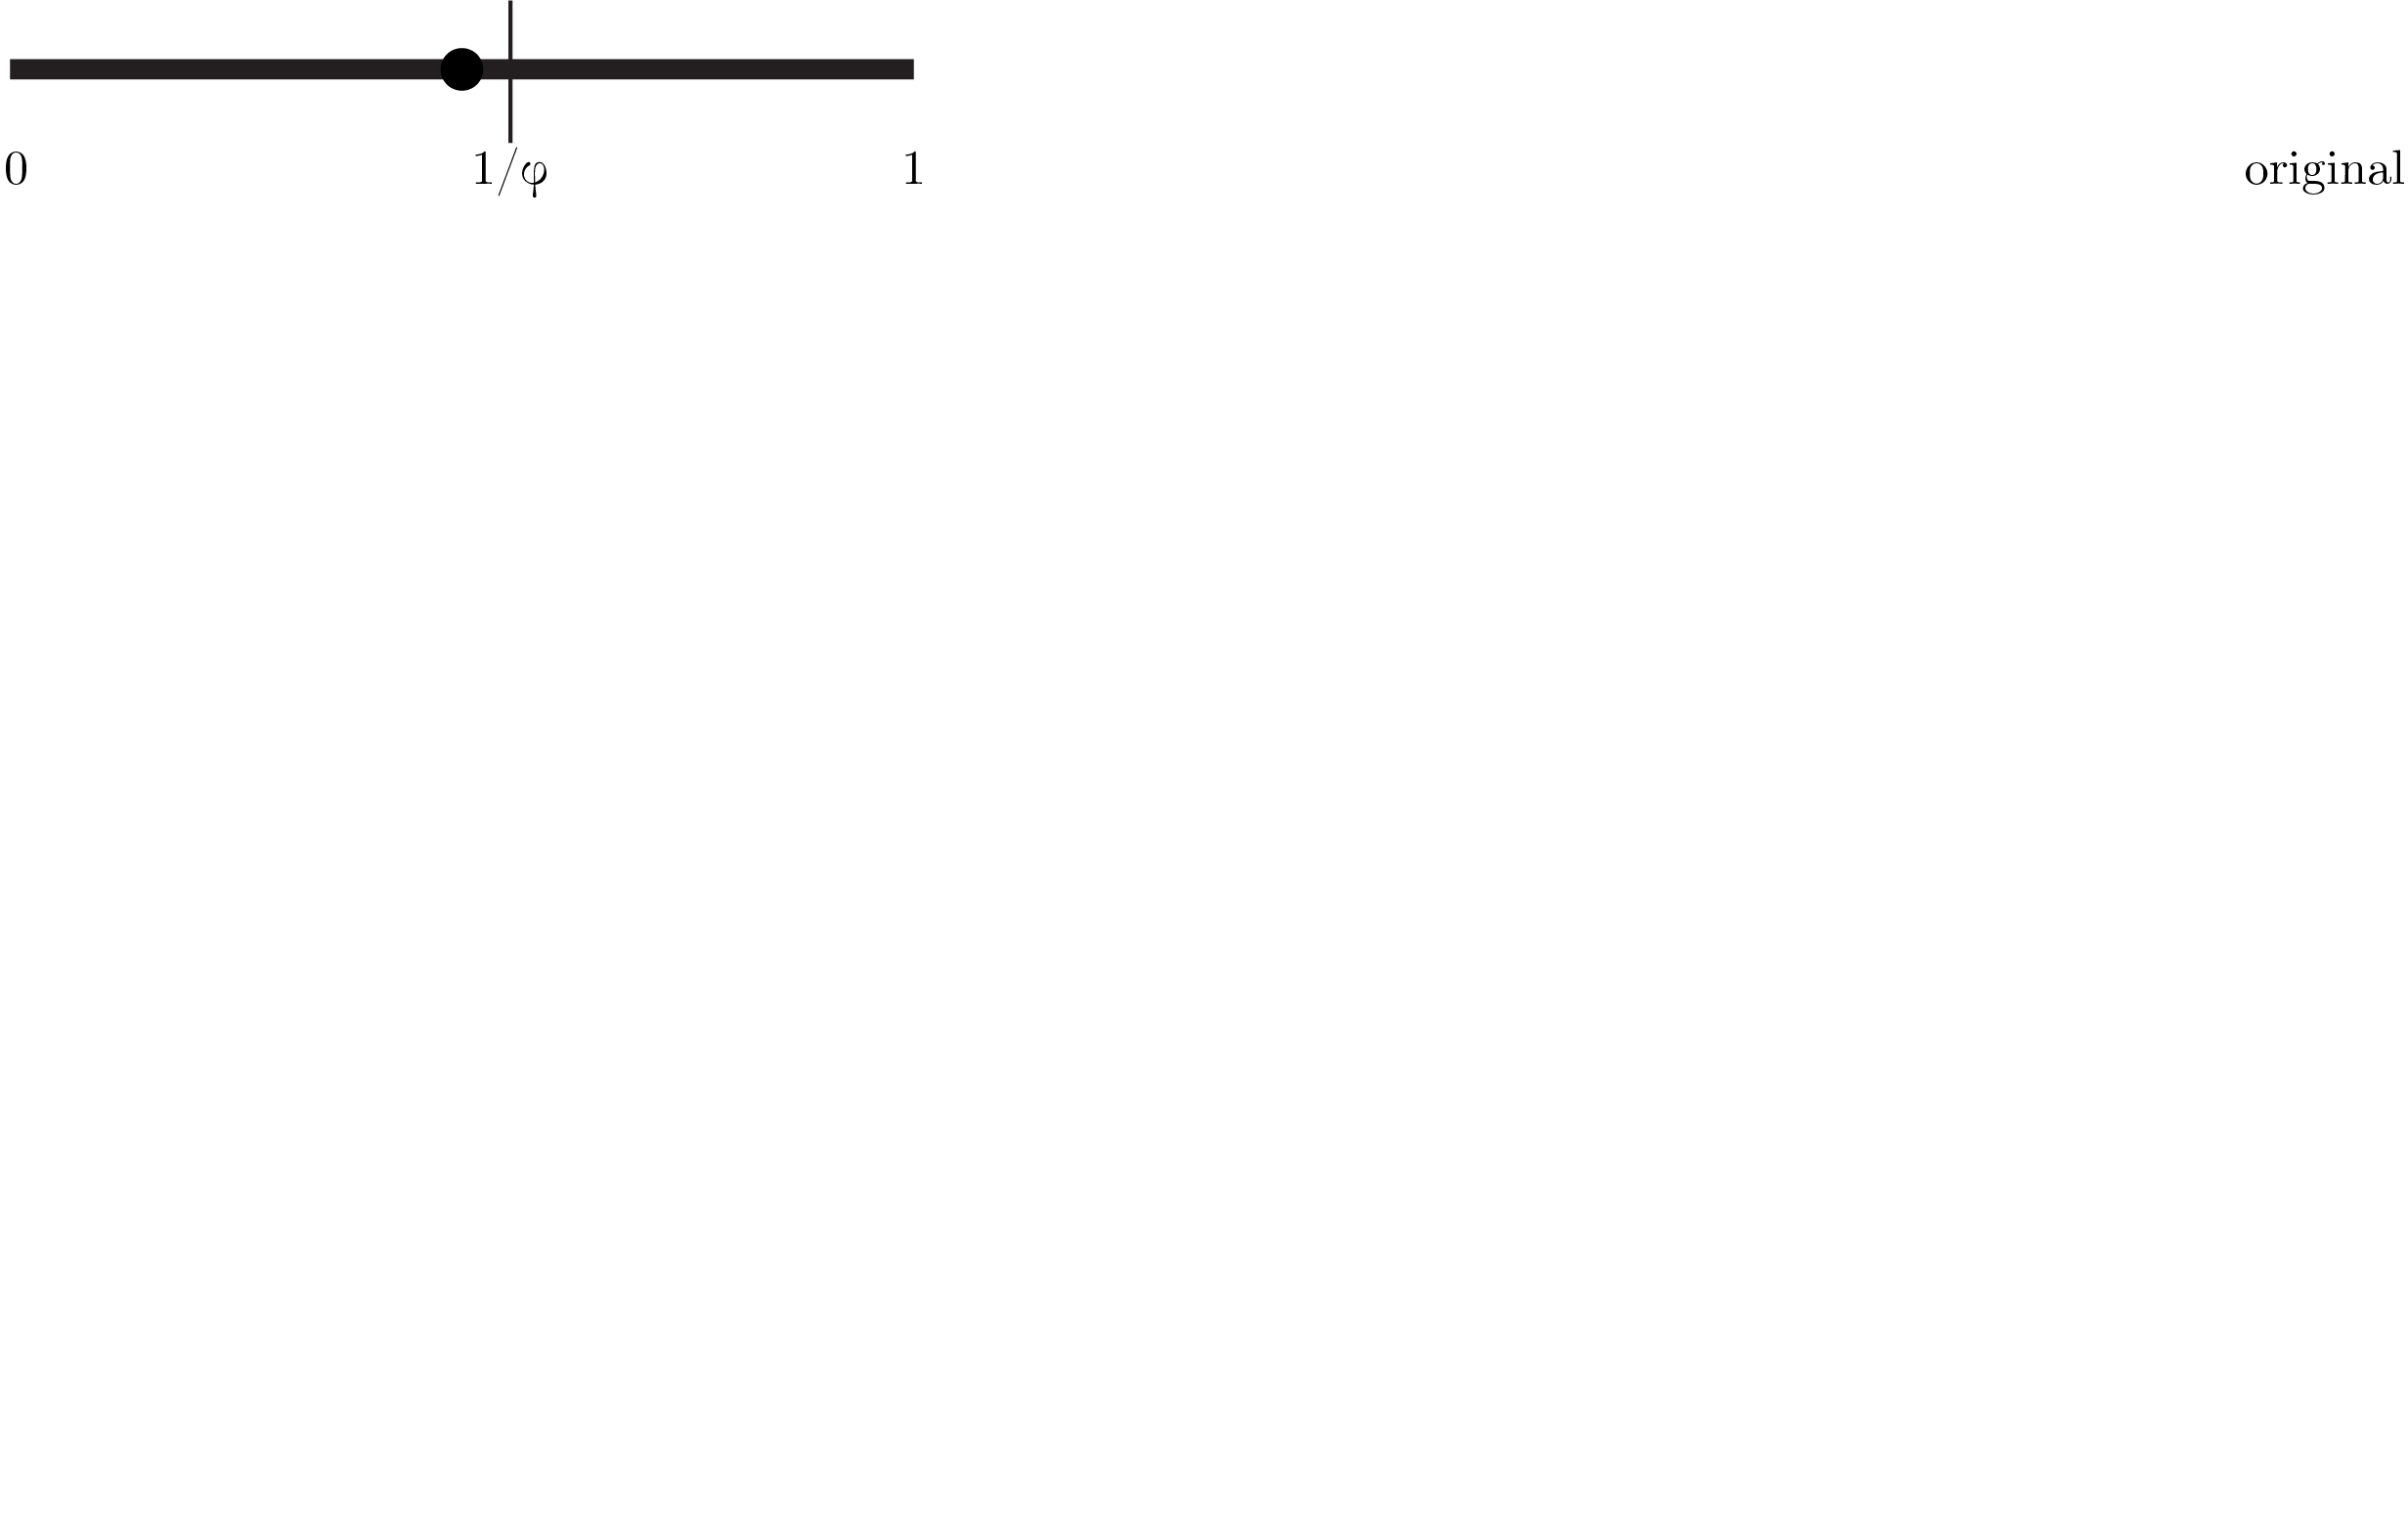
\includegraphics[width=\textwidth,height=0.75\textheight]{images/Phinary/1}
  \end{example}
\end{frame}

\begin{frame}{Dealing with Radix Point Expressions (Geometrically)}
  \addtocounter{framenumber}{-1}
  \begin{example}[Suppose you have a point...]
    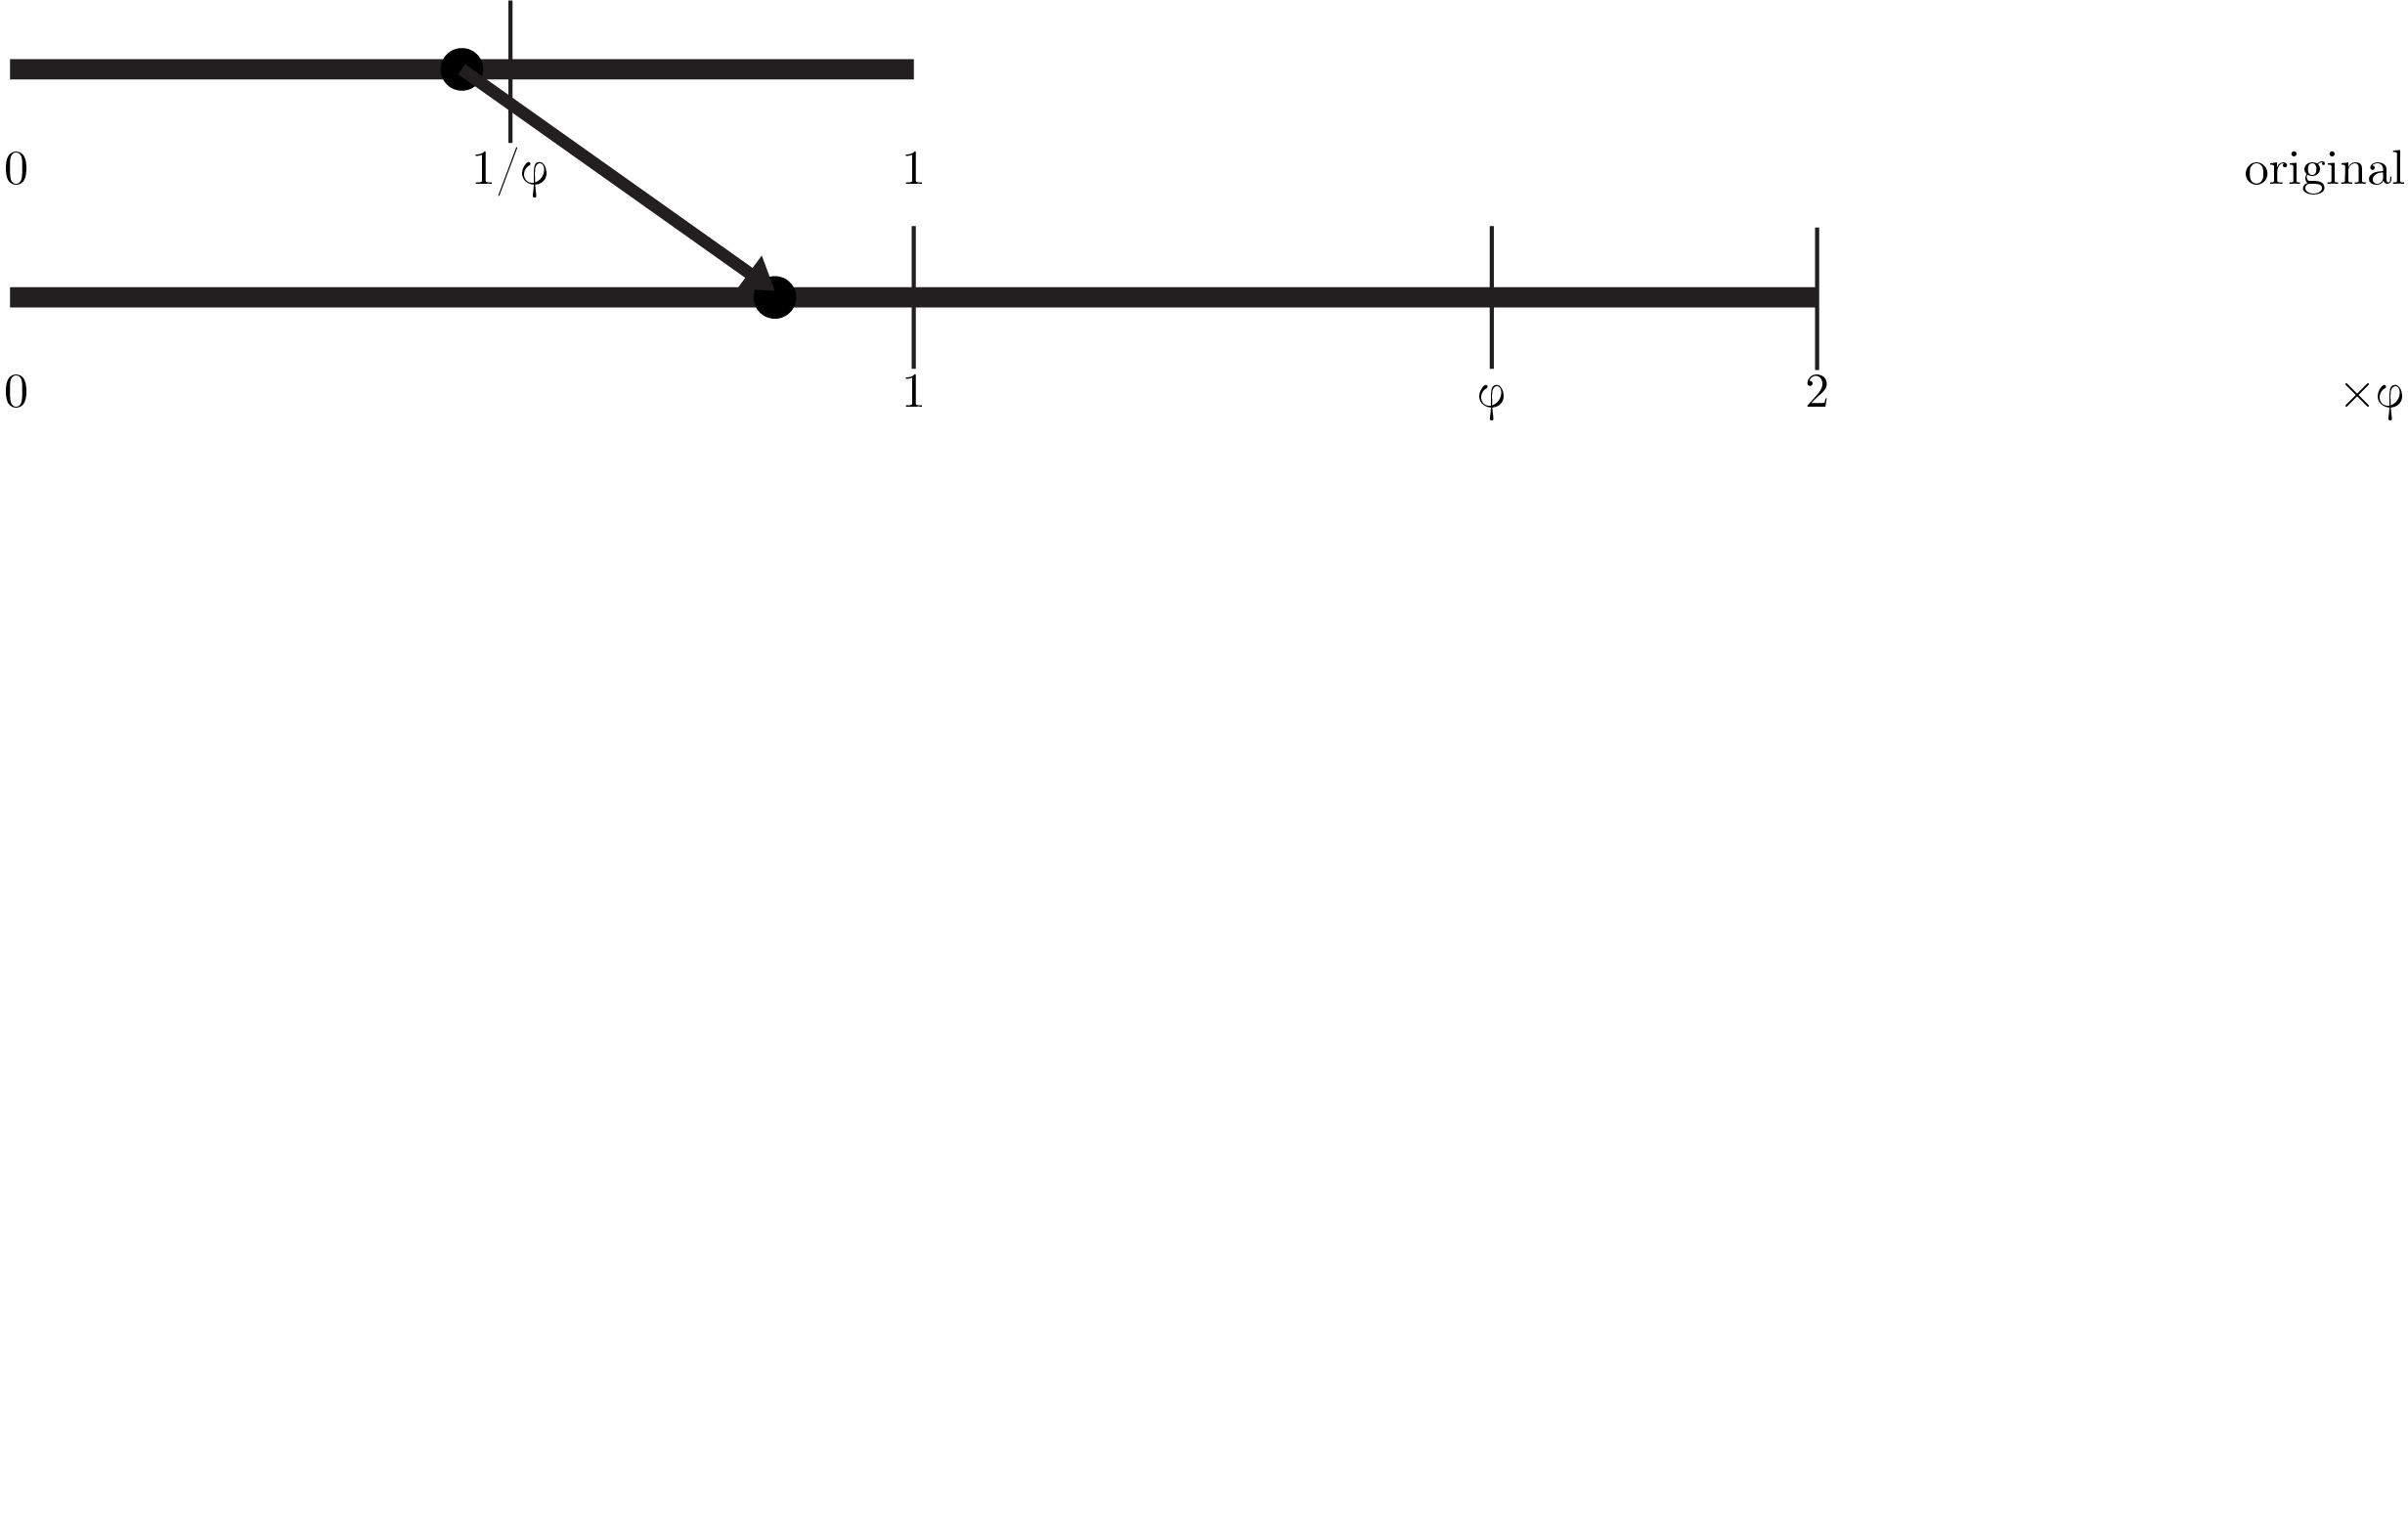
\includegraphics[width=\textwidth,height=0.75\textheight]{images/Phinary/2}
  \end{example}
\end{frame}

\begin{frame}{Dealing with Radix Point Expressions (Geometrically)}
  \addtocounter{framenumber}{-1}
  \begin{example}[Suppose you have a point...]
    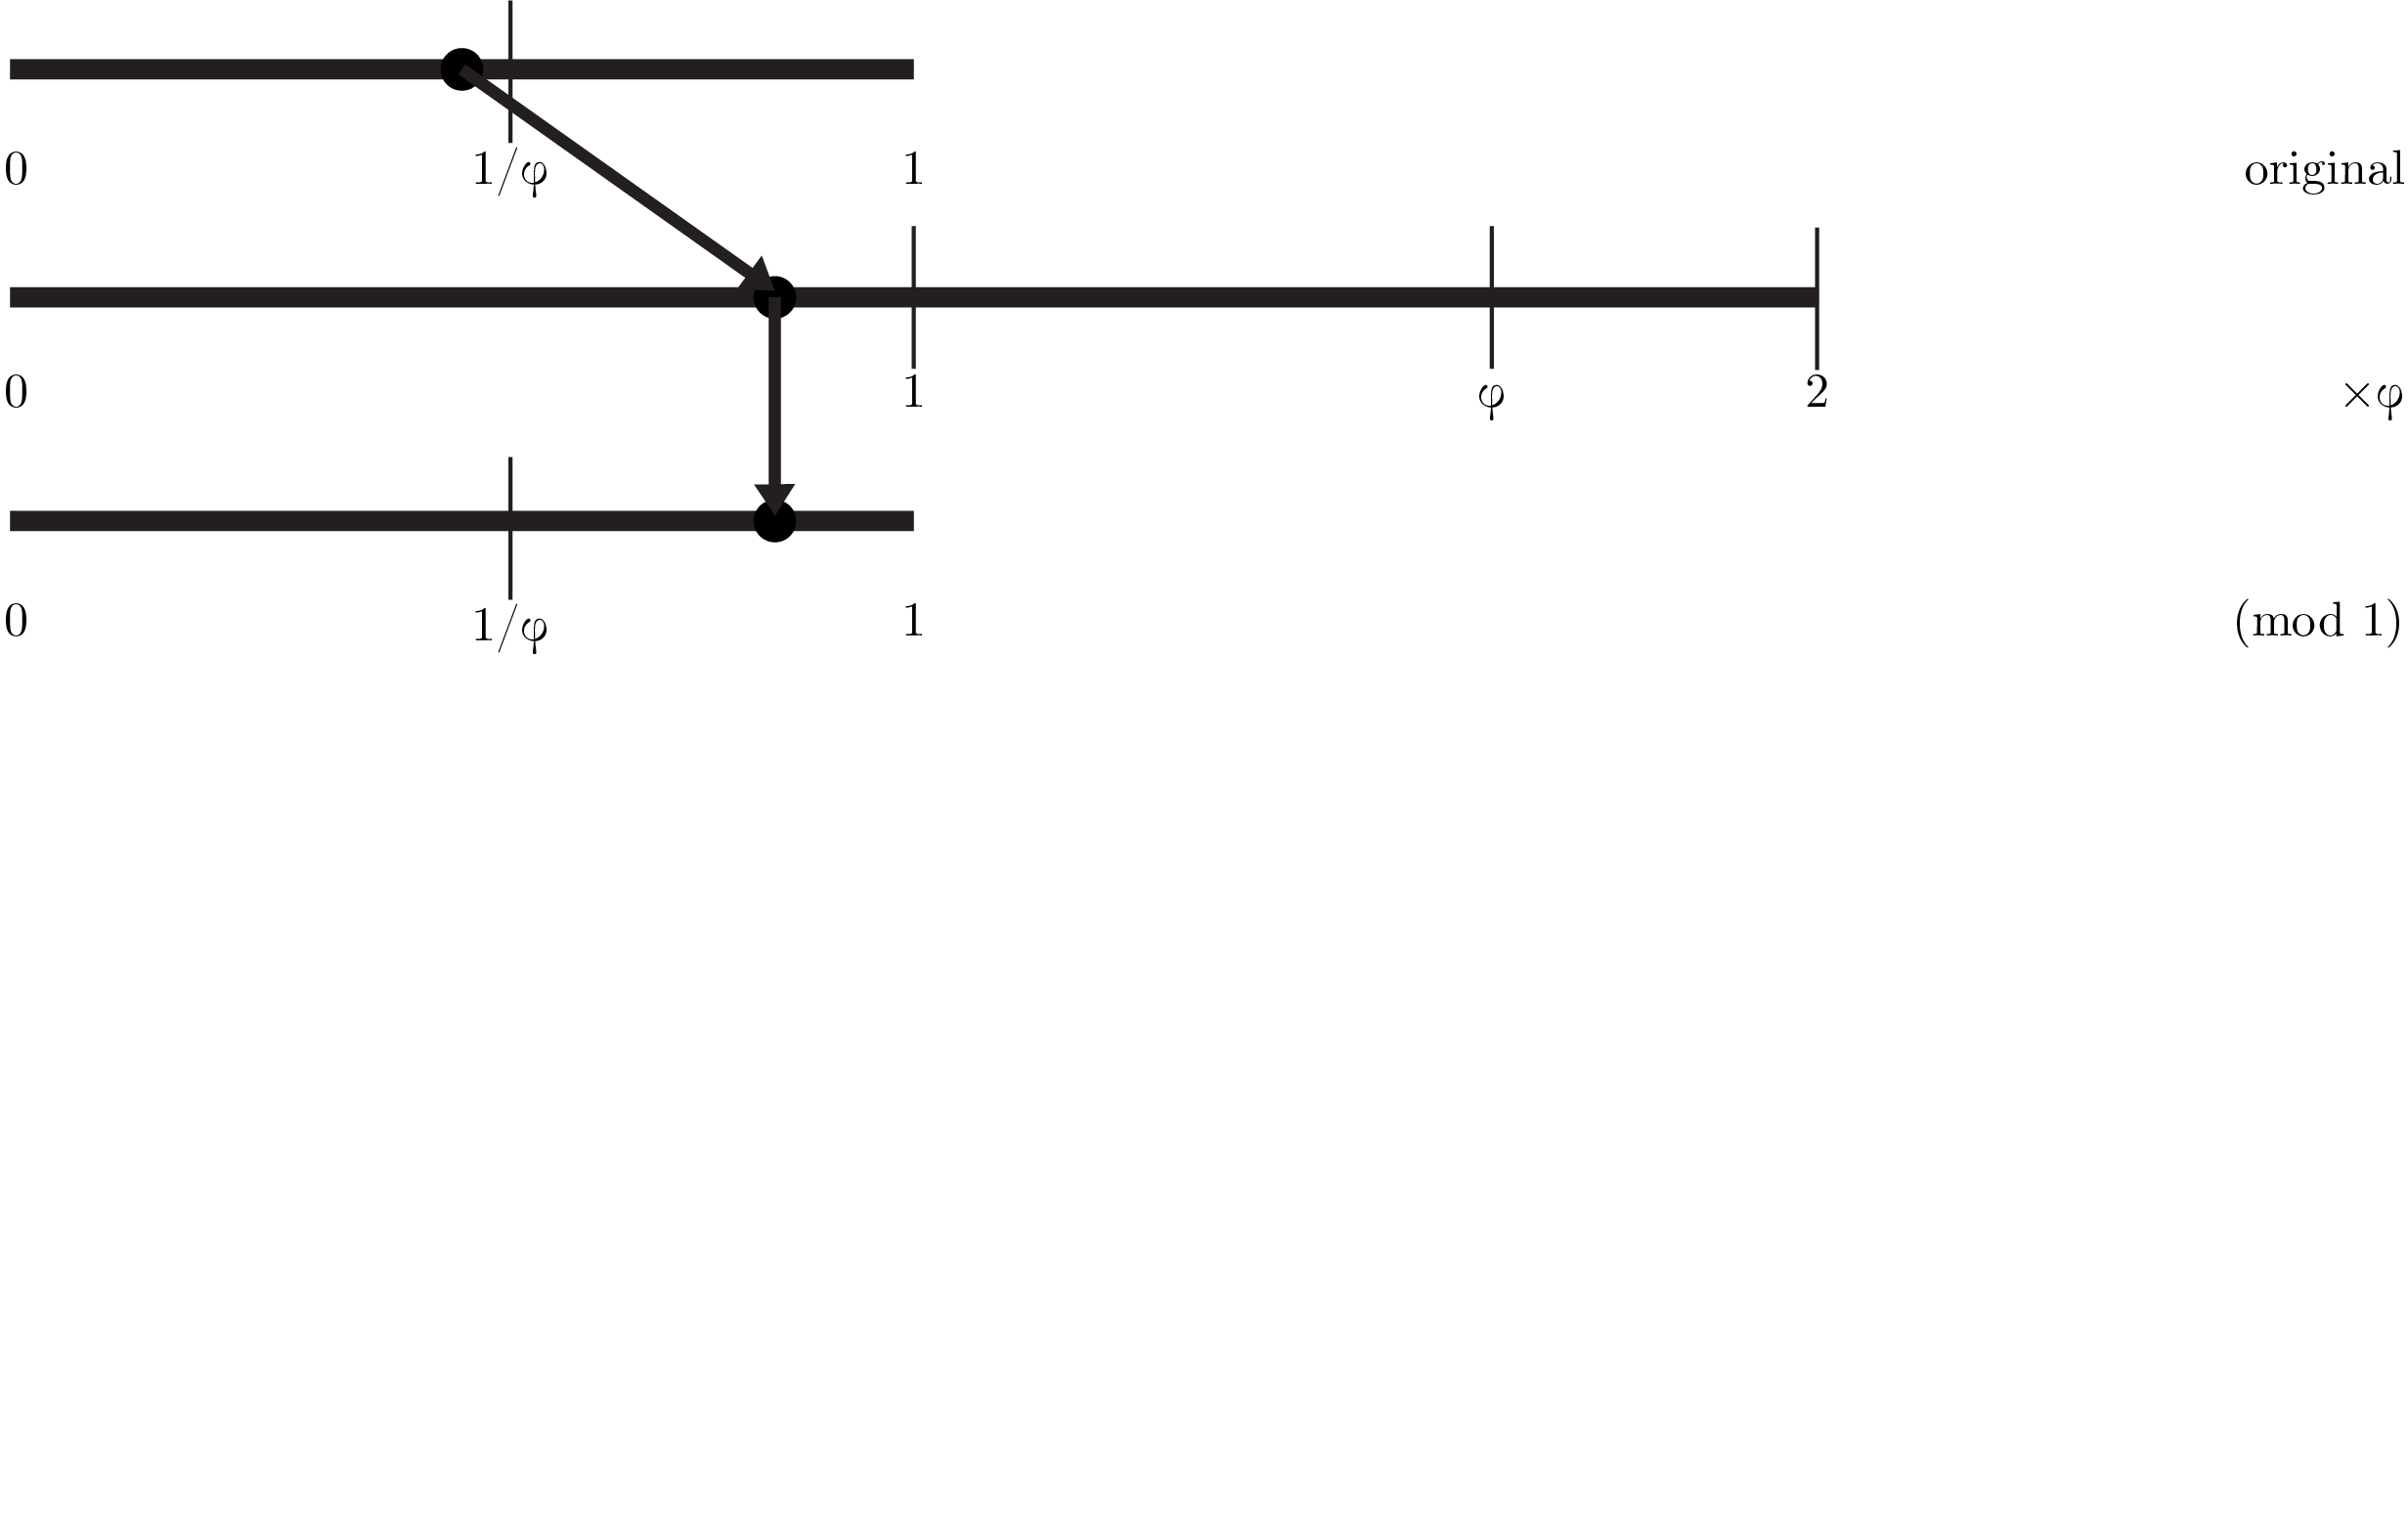
\includegraphics[width=\textwidth,height=0.75\textheight]{images/Phinary/3}
  \end{example}
\end{frame}

\begin{frame}{Dealing with Radix Point Expressions (Geometrically)}
  \addtocounter{framenumber}{-1}
  \begin{example}[Suppose you have a point...]
    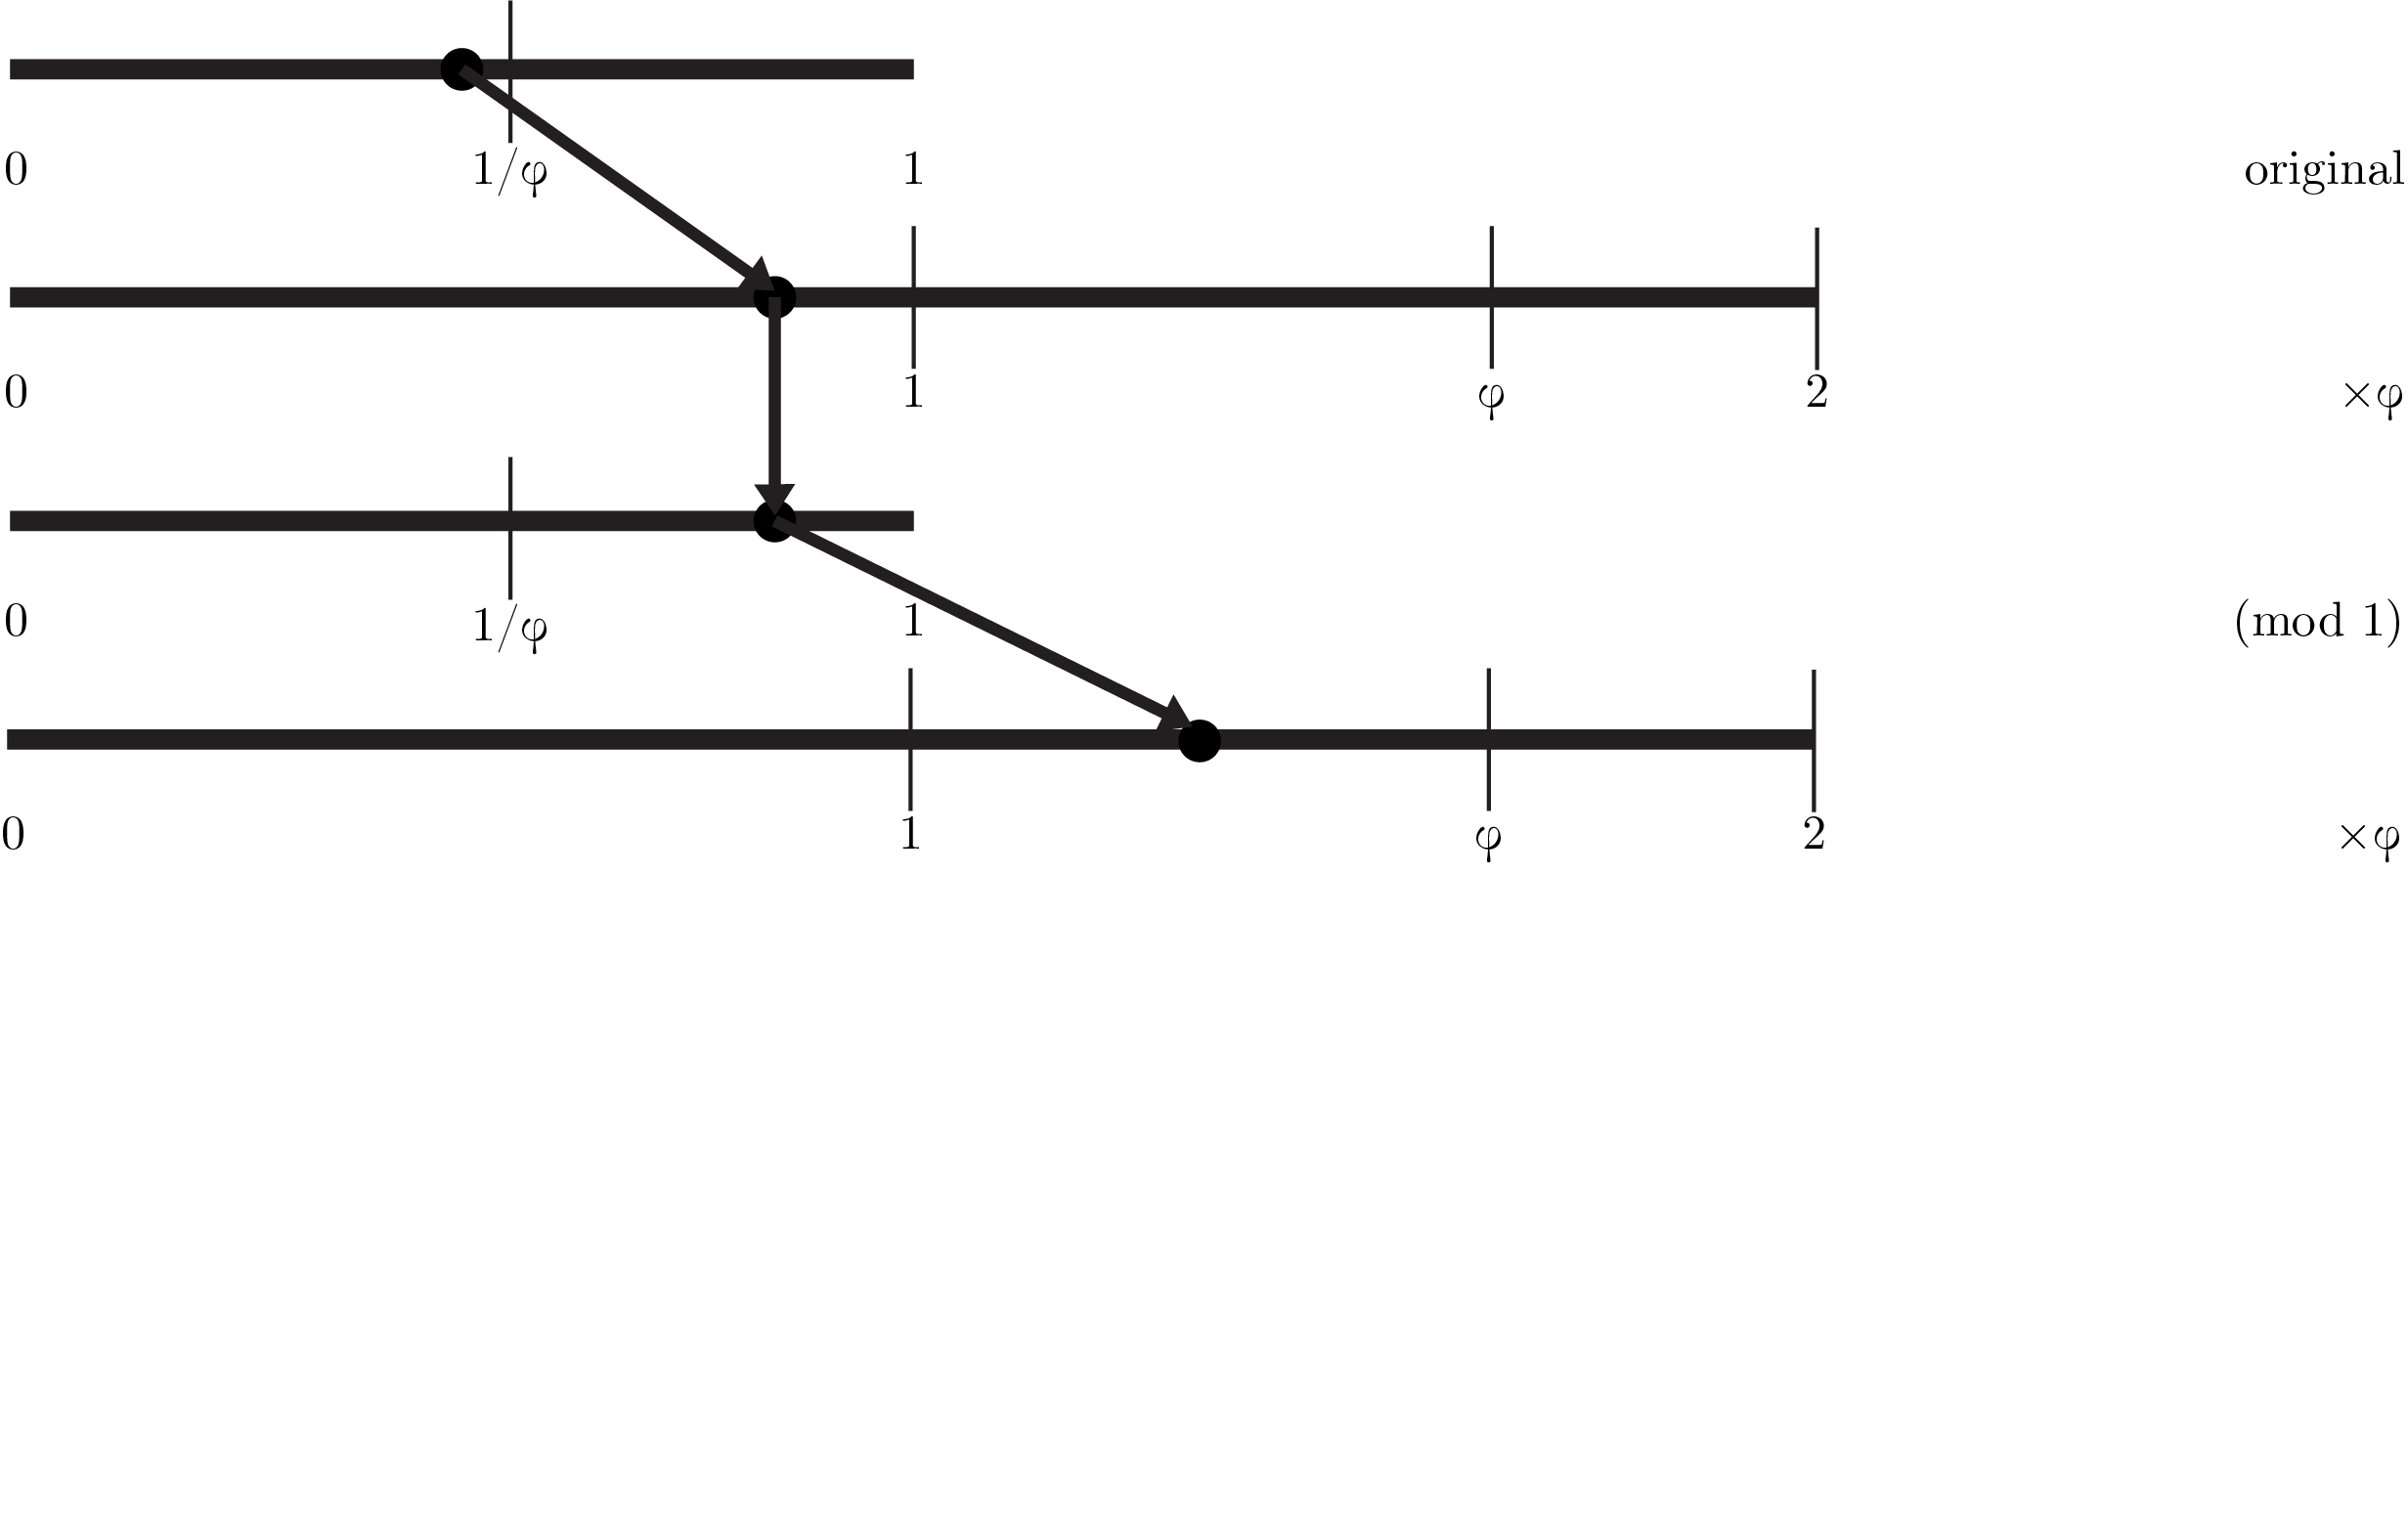
\includegraphics[width=\textwidth,height=0.75\textheight]{images/Phinary/4}
  \end{example}
\end{frame}

\begin{frame}{Dealing with Radix Point Expressions (Geometrically)}
  \addtocounter{framenumber}{-1}
  \begin{example}[Suppose you have a point...]
    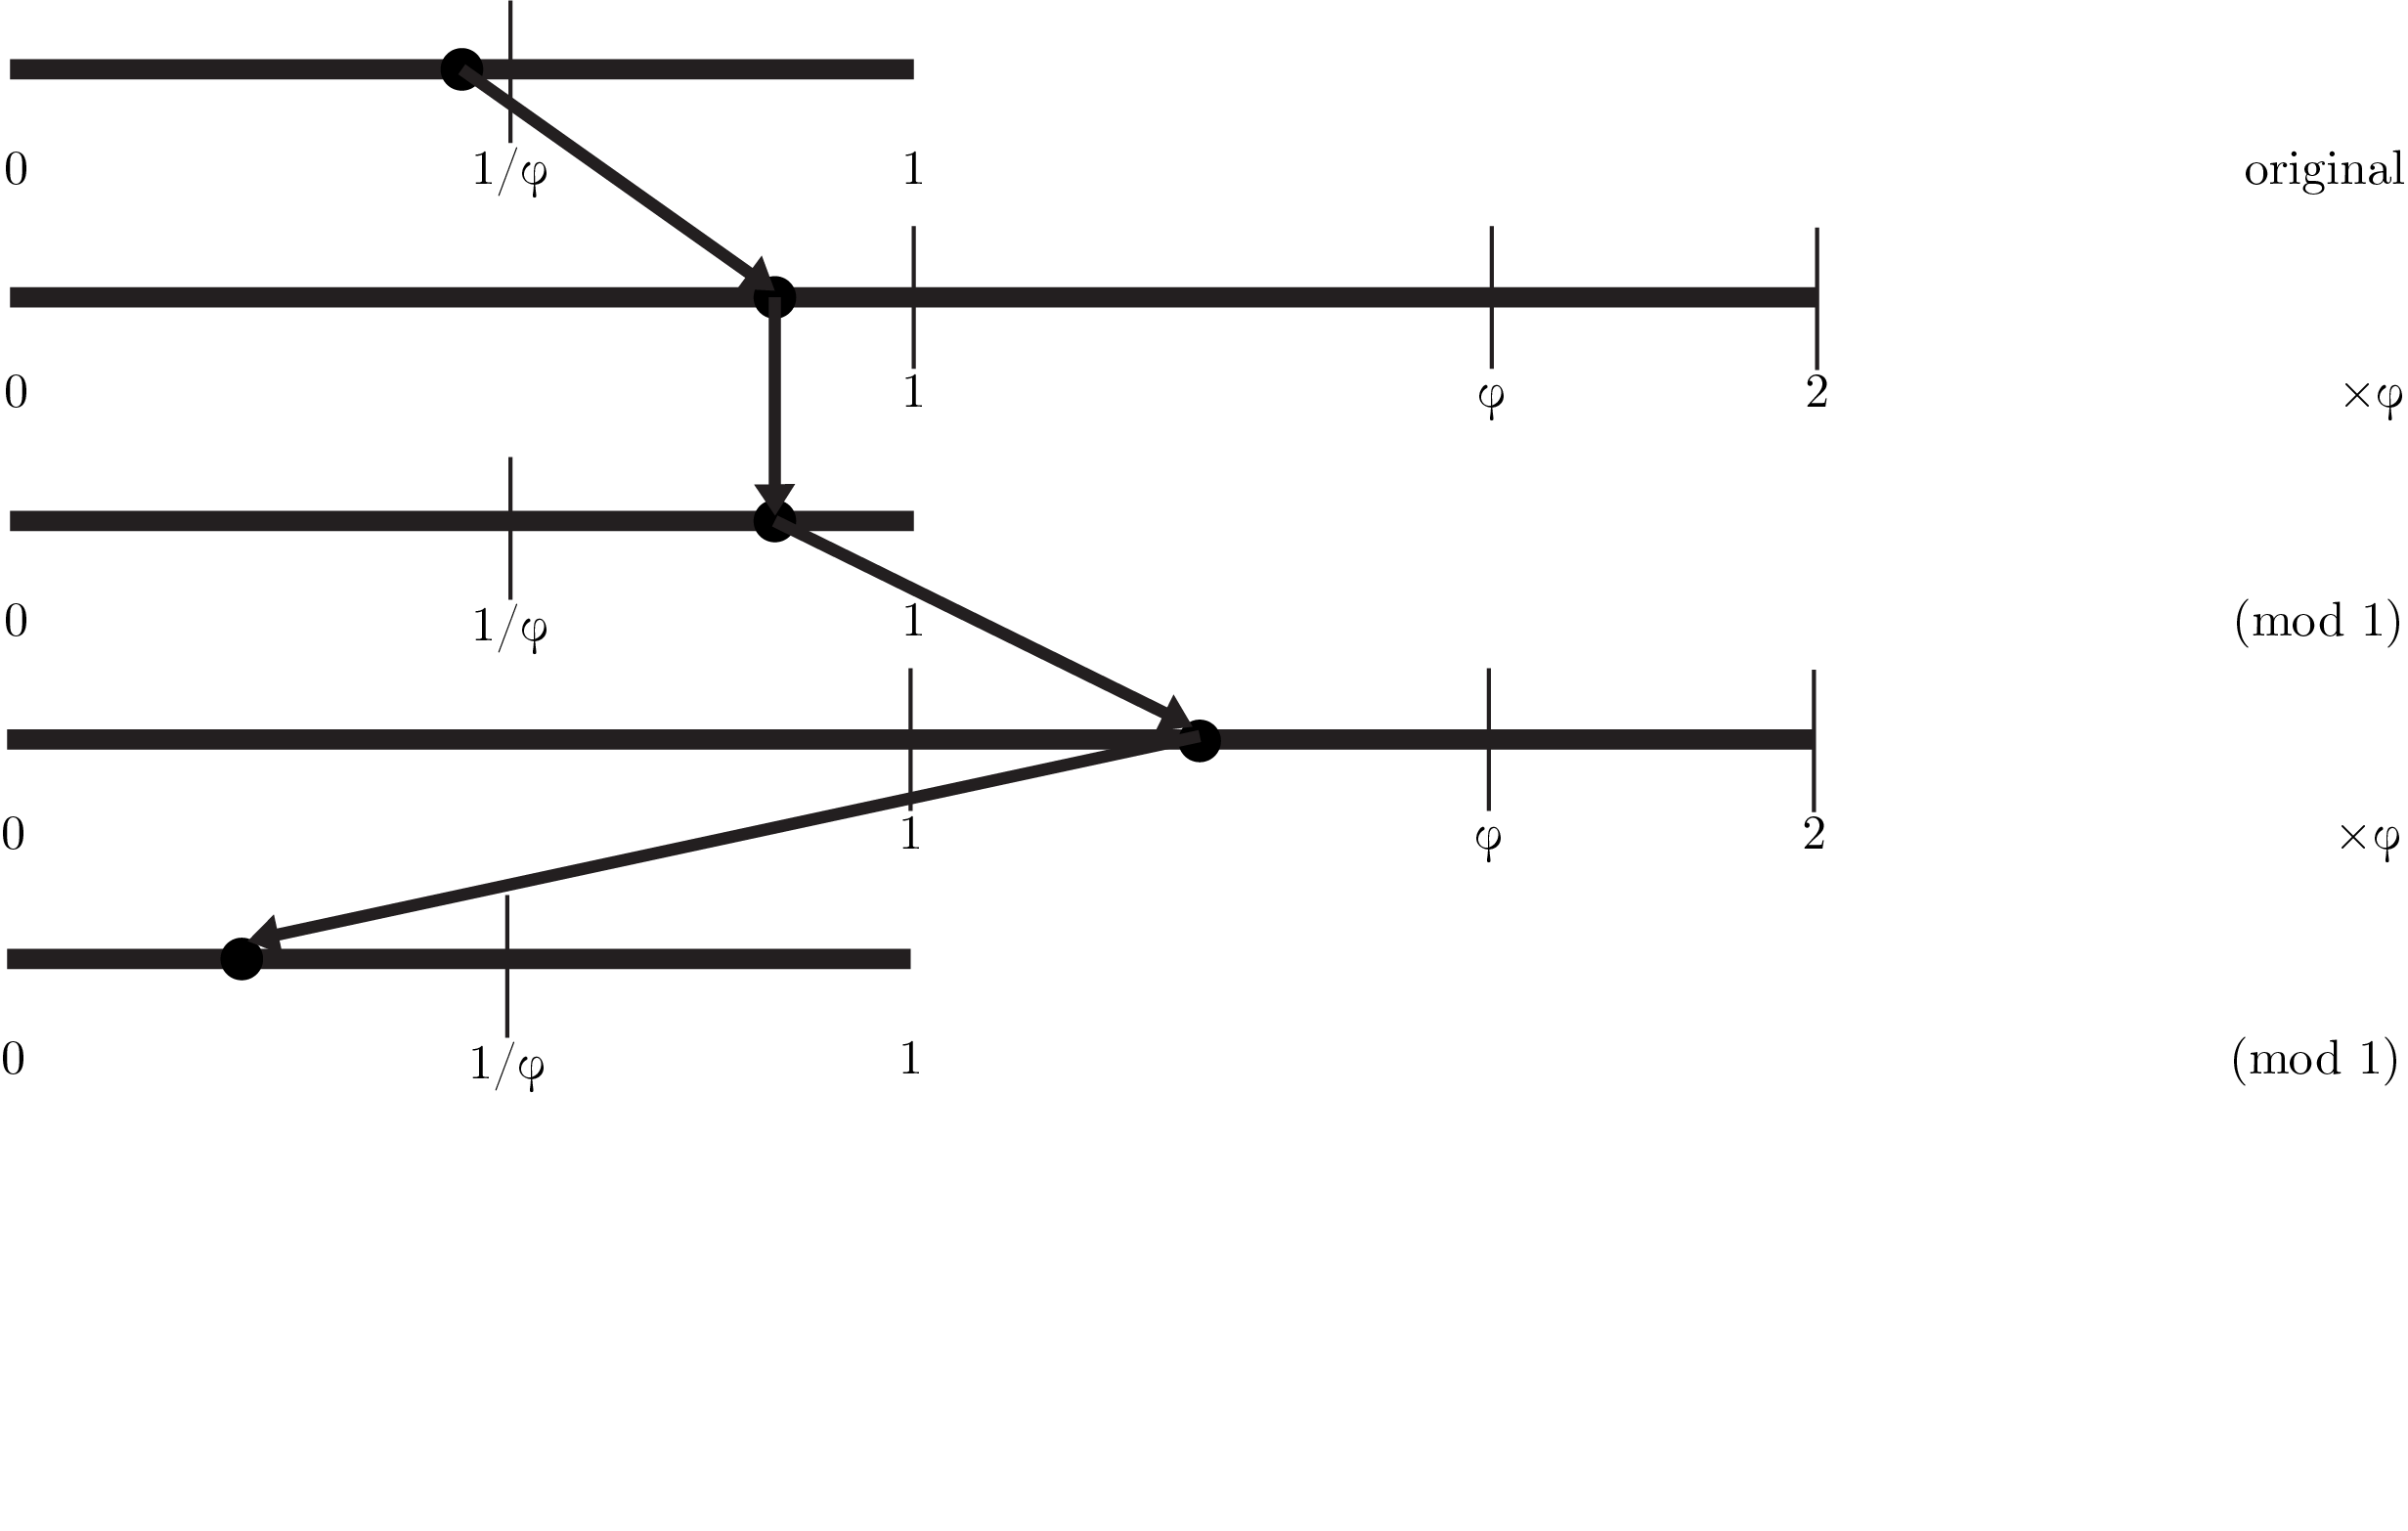
\includegraphics[width=\textwidth,height=0.75\textheight]{images/Phinary/5}
  \end{example}
\end{frame}

\begin{frame}{Dealing with Radix Point Expressions (Geometrically)}
  \addtocounter{framenumber}{-1}
  \begin{example}[Suppose you have a point...]
    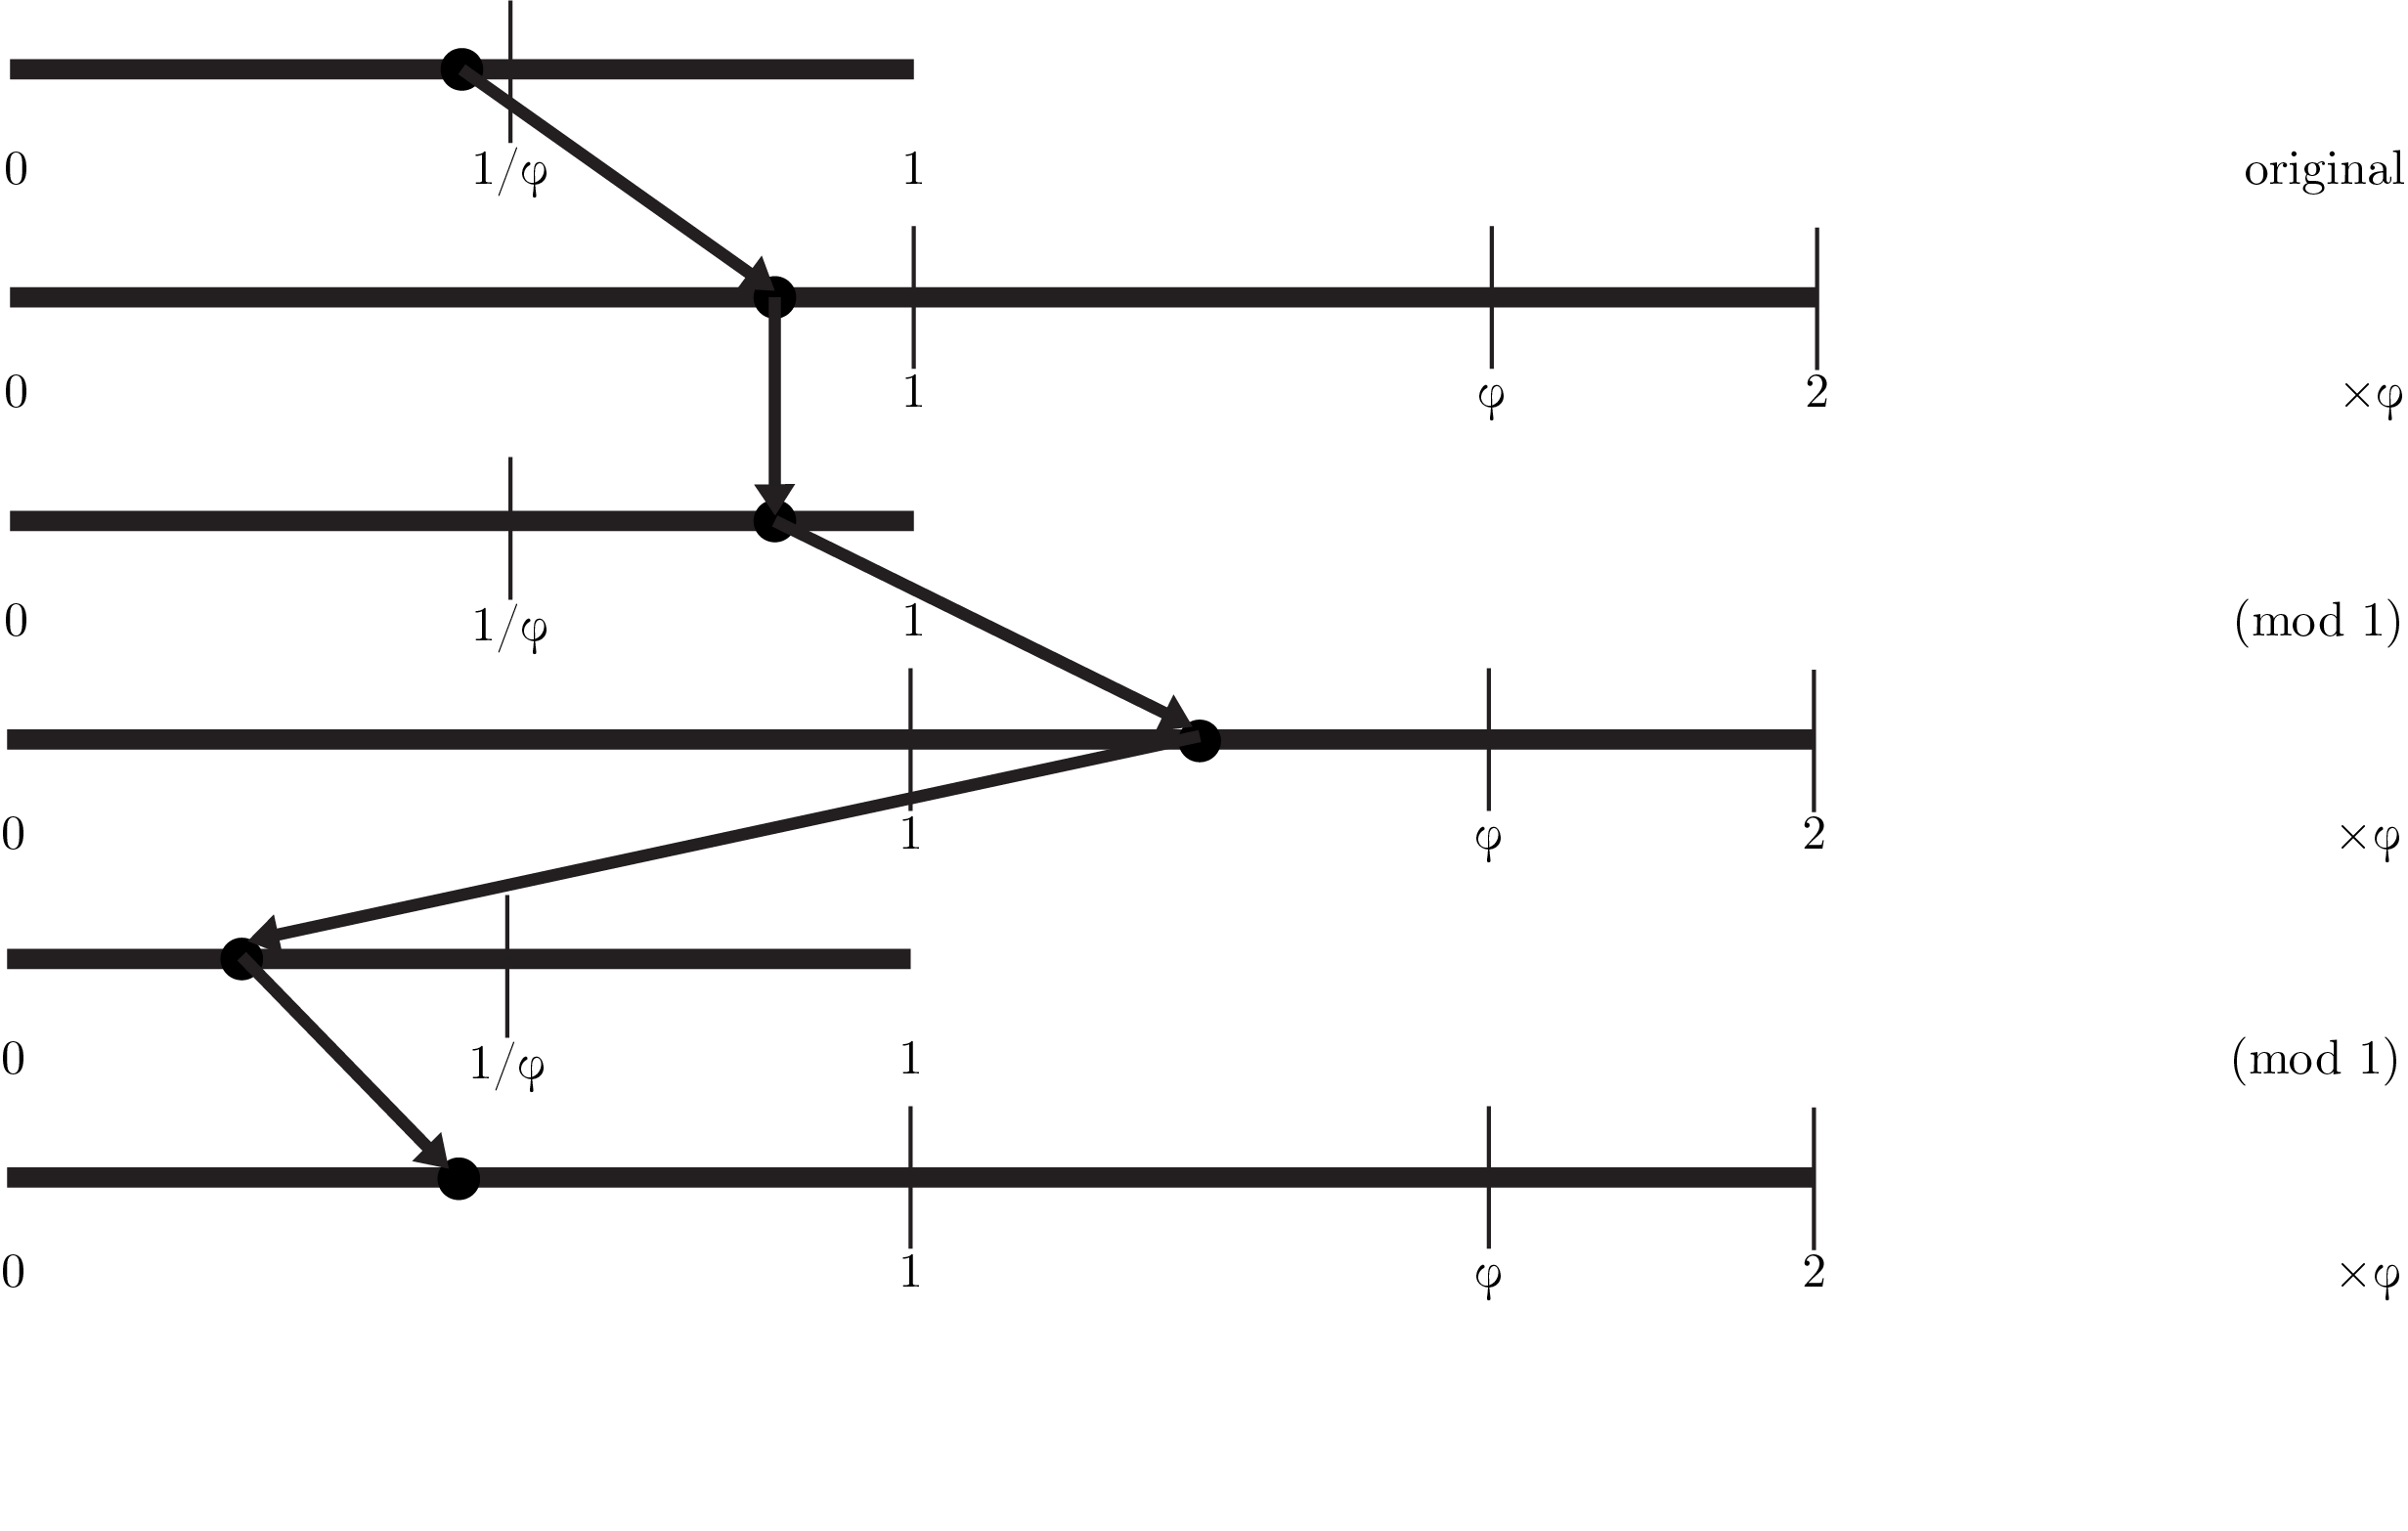
\includegraphics[width=\textwidth,height=0.75\textheight]{images/Phinary/6}
  \end{example}
\end{frame}

\begin{frame}{Dealing with Radix Point Expressions (Geometrically)}
  \addtocounter{framenumber}{-1}
  \begin{example}[Suppose you have a point...]
    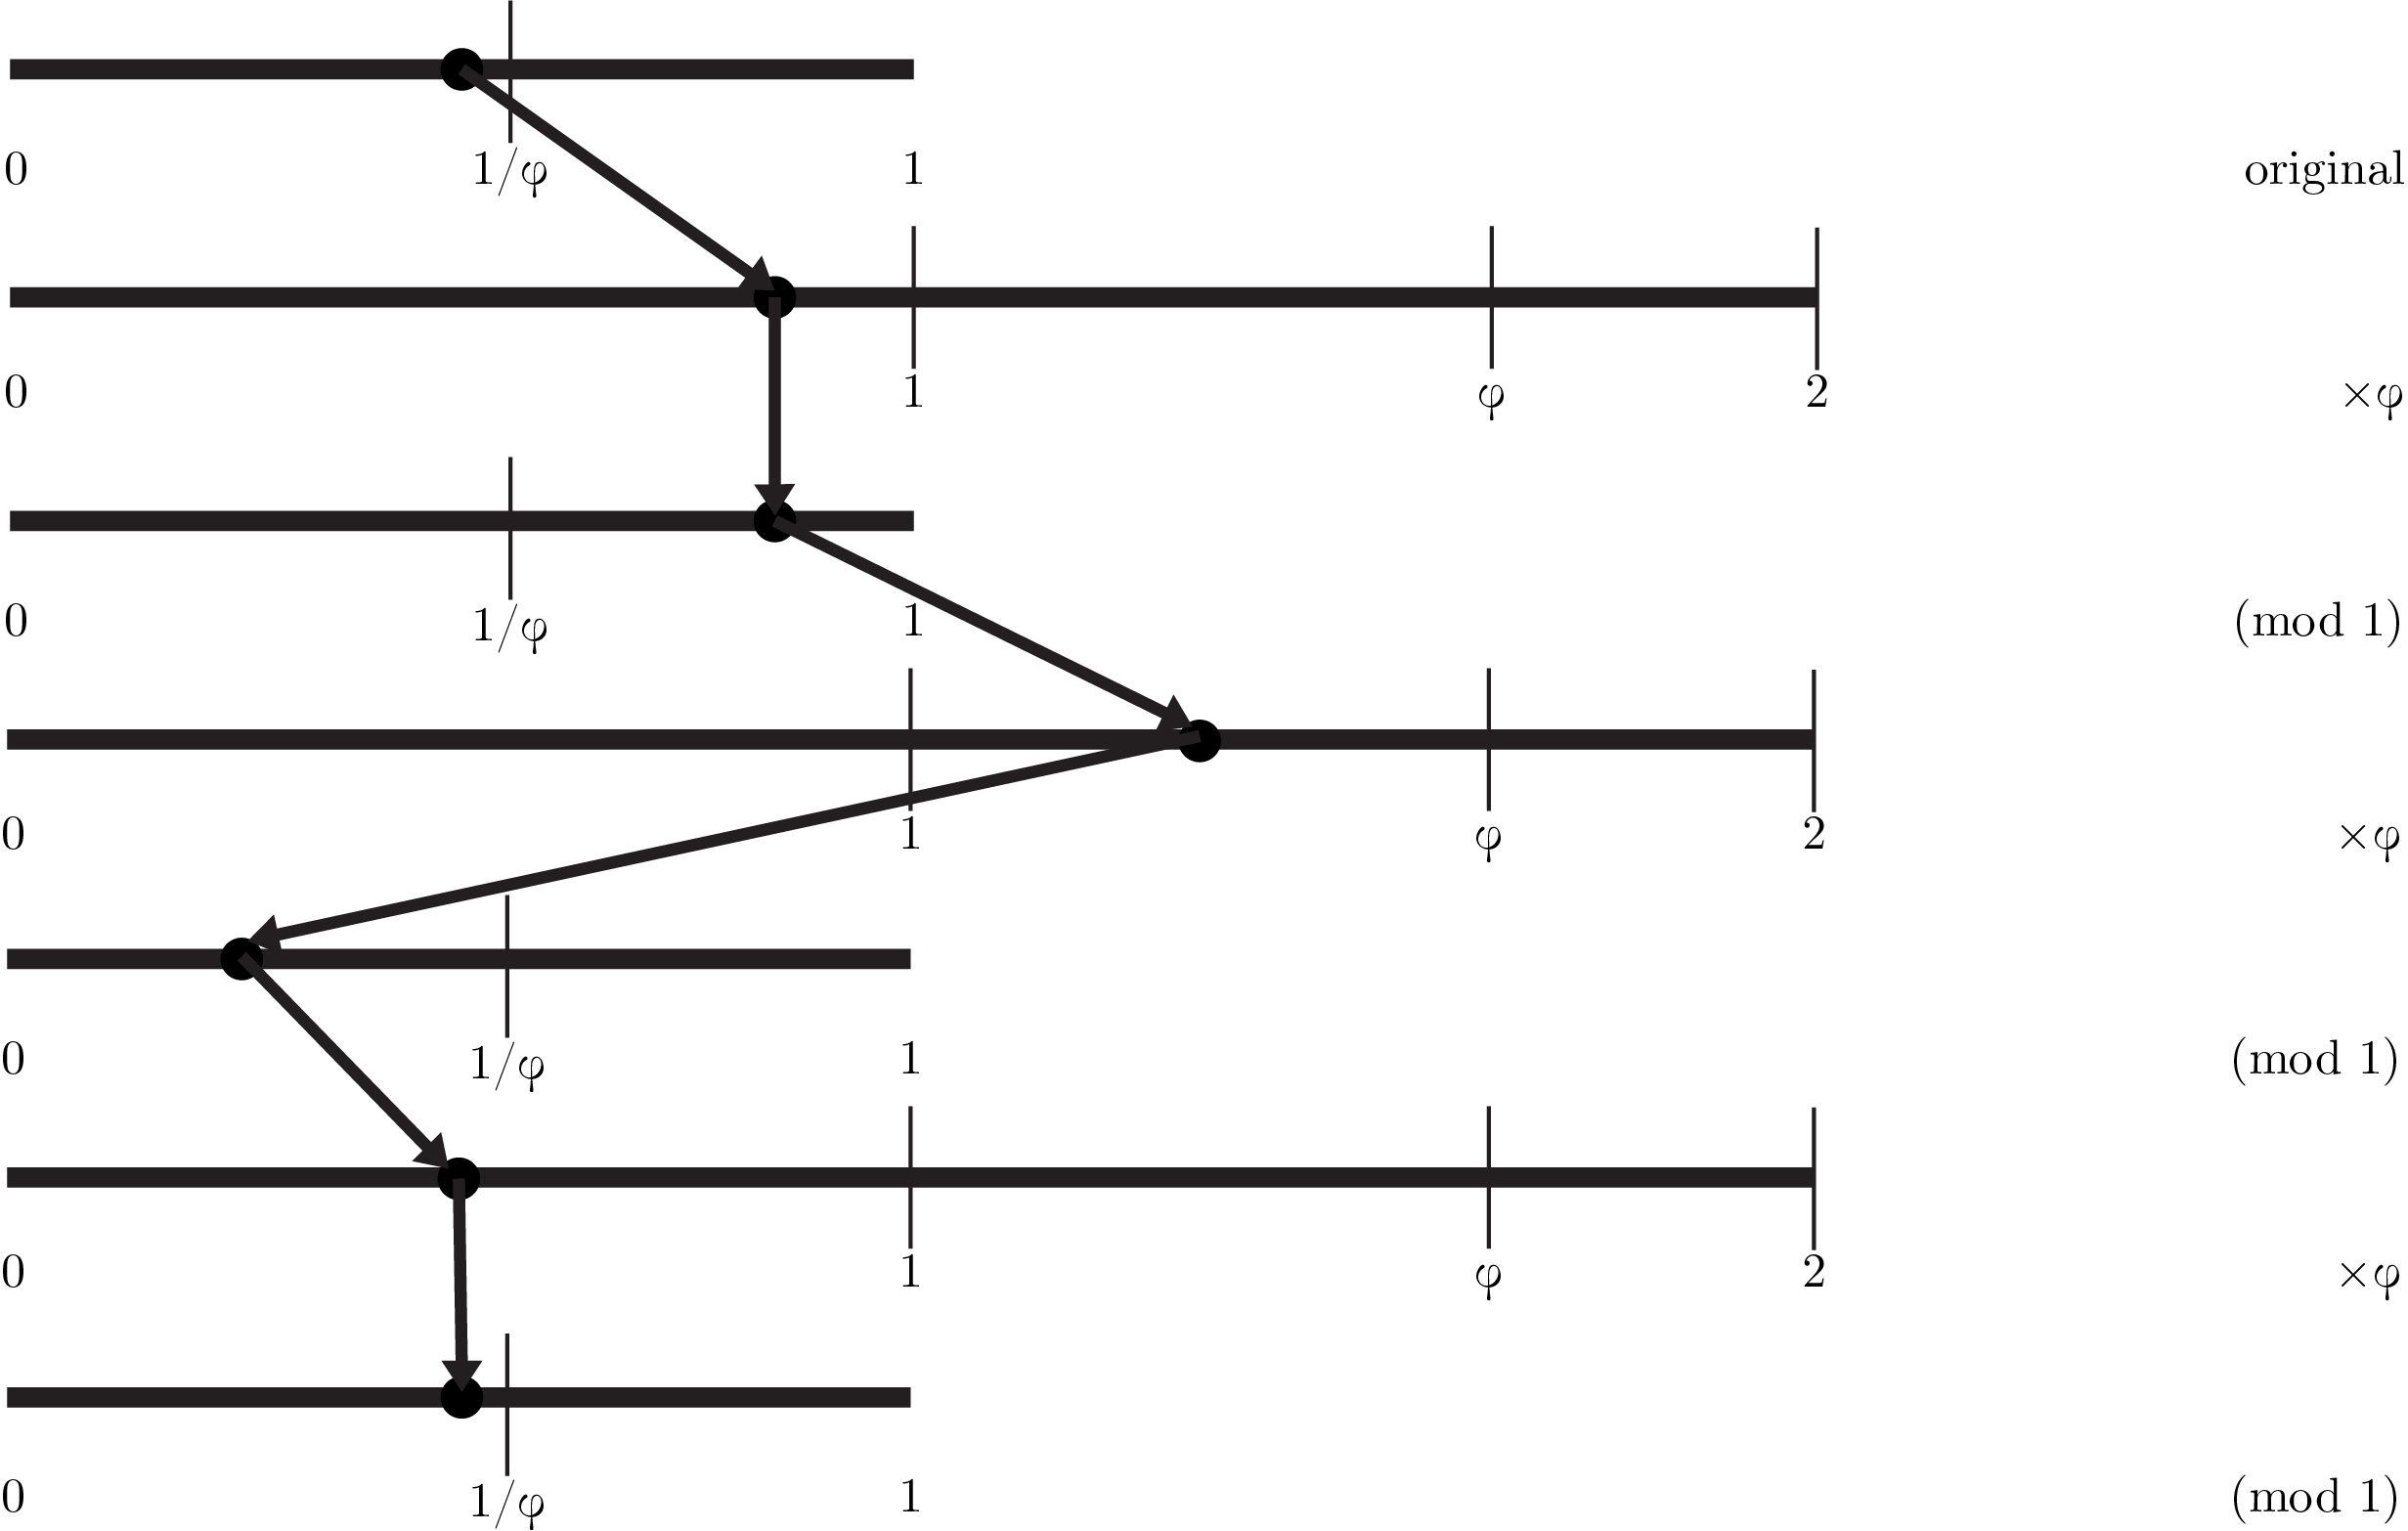
\includegraphics[width=\textwidth,height=0.75\textheight]{images/Phinary/7}
  \end{example}
\end{frame}

\begin{frame}{Dealing with Radix Point Expressions (Geometrically)}
  \addtocounter{framenumber}{-1}
  \begin{example}[Suppose you have a point...]
    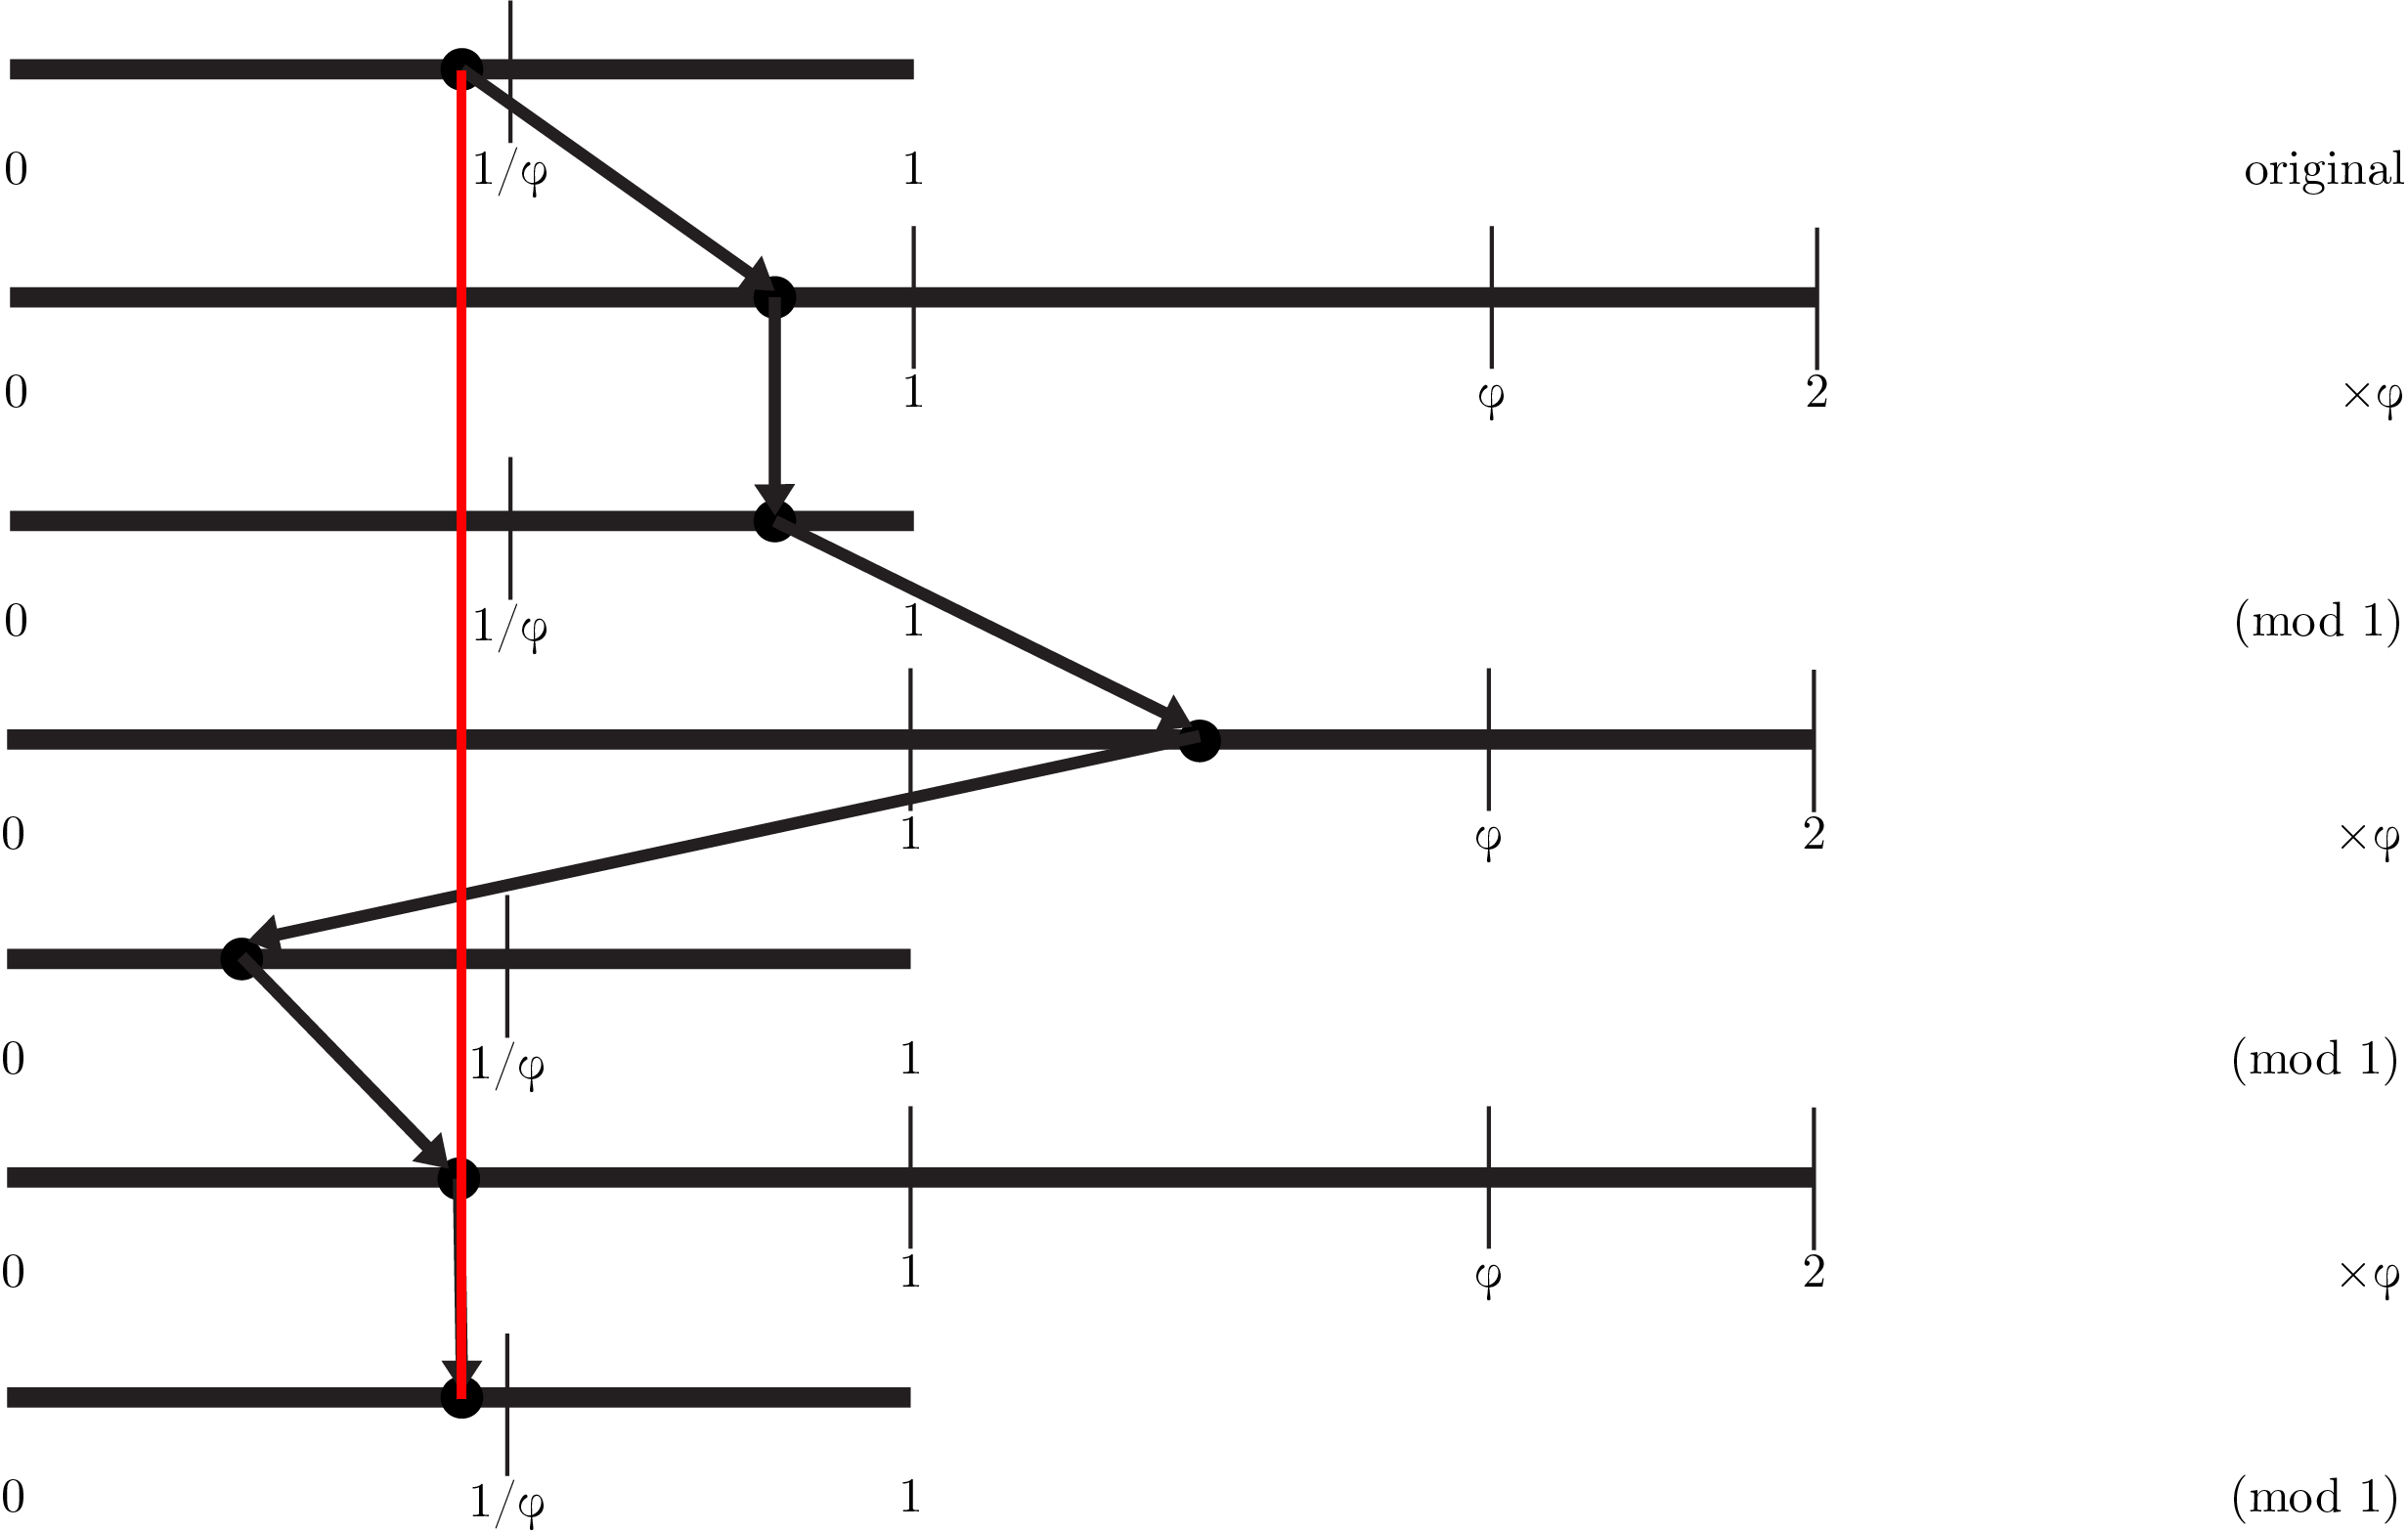
\includegraphics[width=\textwidth,height=0.75\textheight]{images/Phinary/8}
  \end{example}
\end{frame}

\begin{frame}{What this Tells Us}
  \begin{itemize}
    \item Getting stuck in this cycle means this number is not representable as a finite radix point expression in base golden ratio \pause
    \item In general, whole numbers (excluding the base and its multiples) are typically the only numbers with finite representations in non-integer, algebraic bases
  \end{itemize}
\end{frame}

\begin{frame}{Silver Ratio}
  \begin{block}{Silver Ratio}
    The positive solution to the equation $\alpha^2 = 2\alpha + 1$.

    $\alpha = 1+\sqrt{2} \approx 2.414$.
  \end{block}
\end{frame}









%%%%%%%%%%%%%%%%%%%%%%%%%%%%%%%%%%%%%%%%%%%%%%%%%%%%%%%%%%%%%%%%%%
%%        EXAMPLES AND PROPERTIES OF NON-INTEGER BASES          %%
%%%%%%%%%%%%%%%%%%%%%%%%%%%%%%%%%%%%%%%%%%%%%%%%%%%%%%%%%%%%%%%%%%
\subsection{Properties of Non-Integer Bases}
\begin{frame}{Properties of Non-Integer Bases}
  \begin{itemize}
    \item There will be forbidden words \pause
    \begin{itemize}
      \item We can find these by using the orbit of any whole number in these bases (one is the easiest choice) \pause
    \end{itemize}
    \item It is easy/interesting to represent certain numbers in these bases \pause
    \item Arithmetic is more of a pain than usual
  \end{itemize}
\end{frame}

\begin{frame}{Definition}
  \begin{block}{Simplest Form}
    A number is in simplest form if we are unable to rewrite the beta expansion such that it includes a higher power.
  \end{block}
\end{frame}

\begin{frame}{Example of Simplest Form}
  \begin{block}{Simplest Form}
    Let $$\varphi^2 = \varphi + 1.$$ \pause
    Using the positive solution of that equation, $\varphi \approx 1.618$, we can show that $0.11_\varphi = 1.00_\varphi$ by using a beta expansion. \pause
    $$0.11_\varphi = 1\times\varphi^{-1} + 1\times\varphi^{-2} = \frac{1}{\varphi} + \frac{1}{\varphi^2}.$$ \pause
    Then,
    $$\frac{\varphi}{\varphi^2} + \frac{1}{\varphi^2} = \frac{\varphi+1}{\varphi^2},$$\pause
    and by the definition of the base, we can rewrite the numerator:
    $$\frac{\varphi^2}{\varphi^2} = 1_\varphi$$
  \end{block}
\end{frame}


\begin{frame}{Golden Ratio Addition}
  \begin{example}[$1_\varphi + 1_\varphi$]\pause
    $1_\varphi = 0.11\varphi.$\pause

    $1_\varphi + 0.11\varphi = 1.11\varphi = 10.01_\varphi.$\pause

    We can double check this operation by doing a beta expansion and using the definition of the base.\pause

    $10.01_\varphi = 1\times\varphi^1+0\times\varphi^0+0\times\varphi^{-1}+1\times\varphi^{-2}=\varphi + 1/\varphi^2 = (\varphi^2 + 1)/\varphi^2 = 2_{10}.$ \pause

    We can calculate any whole number through this method.
  \end{example}
\end{frame}










%%%%%%%%%%%%%%%%%%%%%%%%%%%%%%%%%%%%%%%%%%%%%%%%%%%%%%%%%%%%%%%%%%
%%             LANGUAGE GENERATED BY NON-INTEGER BASES          %%
%%%%%%%%%%%%%%%%%%%%%%%%%%%%%%%%%%%%%%%%%%%%%%%%%%%%%%%%%%%%%%%%%%
\subsection{Language Generated by Non-Integer Bases}
\begin{frame}{Example of Simplest Form}
  \begin{block}{Simplest Form}
    Let $$\varphi^2 = \varphi + 1.$$
    Using the positive solution of that equation, $\varphi \approx 1.618$, we can show that $0.11_\varphi = 1.00_\varphi$ by using a beta expansion.
    $$0.11_\varphi = 1\times\varphi^{-1} + 1\times\varphi^{-2} = \frac{1}{\varphi} + \frac{1}{\varphi^2}.$$
    Then,
    $$\frac{\varphi}{\varphi^2} + \frac{1}{\varphi^2} = \frac{\varphi+1}{\varphi^2},$$
    and by the definition of the base, we can rewrite the numerator:
    $$\frac{\varphi^2}{\varphi^2} = 1_\varphi$$
  \end{block}
\end{frame}

\begin{frame}{What Makes a Word Forbidden in Non-Integer Bases?}
  \begin{itemize}
    \item In general, a word is forbidden if it is not in simplest form \pause
    \item In actuality, it is because it escapes the range of the beta map
  \end{itemize}
\end{frame}

\begin{frame}{Escaping the Beta Map}
  \begin{example}[Golden Base Ratio: $T(0.011_\varphi)$]
    Using our previous example:
    $$T(0.011_\varphi)=0.11_\varphi=1.00_\varphi.$$ \pause
    But that can't happen! By definition, $T:[0,1)\to[0,1)$. As such, we say that this is a forbidden word. \pause

    Geometrically, this can't happen. If we multiply a number in [0,1) by any number and perform (mod 1), we will never get a number larger than one. It's the arithmetic equivalent of having $x\cdot\beta > \beta,\ x<1$.
  \end{example}
\end{frame}

\begin{frame}{Finding Forbidden Words}
  \begin{itemize}
    \item Take the orbit of one in the base \pause
    \item Find the period of the orbit and take one segment \pause
    \begin{itemize}
      \item Any sequence of numerals greater than the numerals of the period is not allowed
    \end{itemize}
  \end{itemize}
\end{frame}

\begin{frame}{Definition}
  \begin{block}{Orbit}
    The unique, non-terminating radix point representation of a number in any base.
  \end{block}\pause

  \begin{example}[Orbit of One in Different Bases] \pause
    $1_{10} = 0.\overline{99}_{10}$ \pause

    $1_{9} = 0.\overline{88}_{9}$ \pause

    $1_{2} = 0.\overline{11}_{8}$
  \end{example}
\end{frame}

\begin{frame}{Finding Forbidden Words}
  \begin{itemize}
    \item The orbit of one is composed of the maximum allowed numeral in a language \pause
    \item All the forbidden words then will subwords of the orbit, with one added until the word is the maximum numeral lexicographically possible
  \end{itemize}
\end{frame}

\begin{frame}{Language Generated by base Golden Ratio}
  \begin{itemize}
    \item $0.\overline{10}_\varphi$ is the orbit of one in base golden ratio \pause
    \item Since the maximum allowed numeral in the language is 10, we add one and find that the forbidden word is 11 \pause
    \item There can be more than one forbidden word, but since the maximum lexicographically allowed numeral in base golden ratio is 1, we can't add one again \pause
    \item With this in mind, we can now create a finite state machine
  \end{itemize}
\end{frame}

\begin{frame}{FSM For Language Generated by Base Golden Ratio}
  \begin{center}
    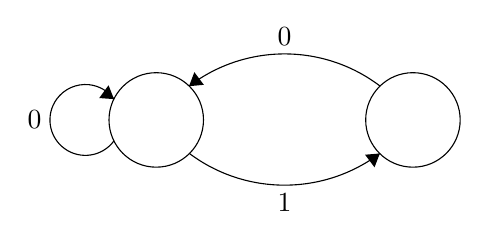
\begin{tikzpicture}[scale=0.2]
      \tikzstyle{every node}+=[inner sep=0pt]
      \draw [black] (33.9,-29.4) circle (3);
      \draw [black] (50.2,-29.4) circle (3);
      \draw [black] (31.22,-30.723) arc (-36:-324:2.25);
      \draw (26.65,-29.4) node [left] {$0$};
      \fill [black] (31.22,-28.08) -- (30.87,-27.2) -- (30.28,-28.01);
      \draw [black] (48.1,-31.527) arc (-53.15335:-126.84665:10.089);
      \fill [black] (48.1,-31.53) -- (47.16,-31.61) -- (47.76,-32.41);
      \draw (42.05,-34.04) node [below] {$1$};
      \draw [black] (35.982,-27.255) arc (127.27809:52.72191:10.019);
      \fill [black] (35.98,-27.26) -- (36.92,-27.17) -- (36.32,-26.37);
      \draw (42.05,-24.71) node [above] {$0$};
    \end{tikzpicture}
  \end{center}
\end{frame}

\begin{frame}{Language Generated by base Silver Ratio}
  \begin{itemize}
    \item $0.\overline{20}_\alpha$ is the orbit of one in base silver ratio \pause
    \item Therefore, 21 and 22 are forbidden words in the language
  \end{itemize}
\end{frame}

\begin{frame}{FSM For Language Generated by Base Silver Ratio}
  \begin{center}
    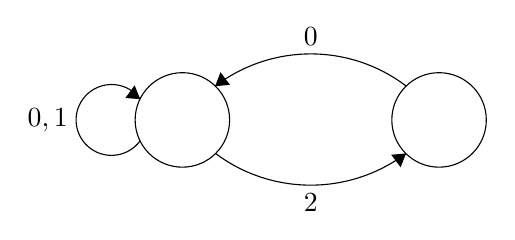
\begin{tikzpicture}[scale=0.2]
      \tikzstyle{every node}+=[inner sep=0pt]
      \draw [black] (33.9,-29.4) circle (3);
      \draw [black] (50.2,-29.4) circle (3);
      \draw [black] (31.22,-30.723) arc (-36:-324:2.25);
      \draw (26.65,-29.4) node [left] {$0,1$};
      \fill [black] (31.22,-28.08) -- (30.87,-27.2) -- (30.28,-28.01);
      \draw [black] (48.1,-31.527) arc (-53.15335:-126.84665:10.089);
      \fill [black] (48.1,-31.53) -- (47.16,-31.61) -- (47.76,-32.41);
      \draw (42.05,-34.04) node [below] {$2$};
      \draw [black] (35.982,-27.255) arc (127.27809:52.72191:10.019);
      \fill [black] (35.98,-27.26) -- (36.92,-27.17) -- (36.32,-26.37);
      \draw (42.05,-24.71) node [above] {$0$};
    \end{tikzpicture}
  \end{center}
\end{frame}
\end{document}
